% !TEX TS-program = xelatex
\documentclass[10pt,landscape,a4paper]{article}
%\usepackage[utf8]{inputenc}
%\usepackage[ngerman]{babel}
\usepackage{graphicx}
\graphicspath{ {./} }
\usepackage{tabularx}
\def\tabularxcolumn#1{m{#1}}
\usepackage{tikz}
\usetikzlibrary{shapes,positioning,arrows,fit,calc,graphs,graphs.standard,trees}
\pgfdeclarelayer{background}
\pgfsetlayers{background,main}
\usepackage[nosf]{kpfonts}
\usepackage[t1]{sourcesanspro}
%\usepackage[lf]{MyriadPro}
%\usepackage[lf,minionint]{MinionPro}
\usepackage{multicol}
\usepackage{wrapfig}
\usepackage[top=0mm,bottom=1mm,left=0mm,right=1mm]{geometry}
\usepackage[framemethod=tikz]{mdframed}
\usepackage{microtype}
%\usepackage{physics}
\usepackage{cancel, mathtools}
\usepackage{lastpage}
\usepackage{datetime}
\yyyymmdddate
\renewcommand{\dateseparator}{-}
\let\bar\overline

\definecolor{myblue}{cmyk}{1,.72,0,.38}

\def\firstcircle{(0,0) circle (1.5cm)}
\def\secondcircle{(0:2cm) circle (1.5cm)}

\colorlet{circle edge}{myblue}
\colorlet{circle area}{myblue!5}

\tikzset{filled/.style={fill=circle area, draw=circle edge, thick},
    outline/.style={draw=circle edge, thick}}

\pgfdeclarelayer{background}
\pgfsetlayers{background,main}

\everymath\expandafter{\the\everymath \color{myblue}}
%\everydisplay\expandafter{\the\everydisplay \color{myblue}}


\renewcommand{\baselinestretch}{.8}
\pagestyle{empty}

\global\mdfdefinestyle{header}{%
linecolor=gray,linewidth=1pt,%
leftmargin=0mm,rightmargin=0mm,skipbelow=0mm,skipabove=0mm,
}

\newcommand{\header}{
\begin{mdframed}[style=header]
\footnotesize
\sffamily
CS1231 Finals Cheatsheet v1.0 (\today)\\
by~Julius~Putra~Tanu~Setiaji,~page~\thepage~of~\pageref{LastPage}
\end{mdframed}
}
%\usepackage{chngcntr}

\counterwithin*{equation}{section}
\counterwithin*{equation}{subsection}
\usepackage{enumitem}
\newlist{legal}{enumerate}{10}
\setlist[legal]{label*=\arabic*.,leftmargin=4mm}
\setlist[itemize]{leftmargin=4mm}
\setlist{itemsep=1mm}
\newenvironment{descitemize} % a mixture of description and itemize
{\begin{description}[leftmargin=*,before=\let\makelabel\descitemlabel]}
	{\end{description}}

\newcommand{\descitemlabel}[1]{%
	\textbullet\ \textbf{#1}%
}
\makeatletter



\renewcommand{\section}{\@startsection{section}{1}{0mm}%
                                {.2ex}%
                                {.2ex}%x
                                {\color{myblue}\sffamily\small\bfseries}}
\renewcommand{\subsection}{\@startsection{subsection}{1}{0mm}%
                                {.2ex}%
                                {.2ex}%x
                                {\sffamily\bfseries}}



\def\multi@column@out{%
   \ifnum\outputpenalty <-\@M
   \speci@ls \else
   \ifvoid\colbreak@box\else
     \mult@info\@ne{Re-adding forced
               break(s) for splitting}%
     \setbox\@cclv\vbox{%
        \unvbox\colbreak@box
        \penalty-\@Mv\unvbox\@cclv}%
   \fi
   \splittopskip\topskip
   \splitmaxdepth\maxdepth
   \dimen@\@colroom
   \divide\skip\footins\col@number
   \ifvoid\footins \else
      \leave@mult@footins
   \fi
   \let\ifshr@kingsaved\ifshr@king
   \ifvbox \@kludgeins
     \advance \dimen@ -\ht\@kludgeins
     \ifdim \wd\@kludgeins>\z@
        \shr@nkingtrue
     \fi
   \fi
   \process@cols\mult@gfirstbox{%
%%%%% START CHANGE
\ifnum\count@=\numexpr\mult@rightbox+2\relax
          \setbox\count@\vsplit\@cclv to \dimexpr \dimen@-1cm\relax
\setbox\count@\vbox to \dimen@{\vbox to 1cm{\header}\unvbox\count@\vss}%
\else
      \setbox\count@\vsplit\@cclv to \dimen@
\fi
%%%%% END CHANGE
            \set@keptmarks
            \setbox\count@
                 \vbox to\dimen@
                  {\unvbox\count@
                   \remove@discardable@items
                   \ifshr@nking\vfill\fi}%
           }%
   \setbox\mult@rightbox
       \vsplit\@cclv to\dimen@
   \set@keptmarks
   \setbox\mult@rightbox\vbox to\dimen@
          {\unvbox\mult@rightbox
           \remove@discardable@items
           \ifshr@nking\vfill\fi}%
   \let\ifshr@king\ifshr@kingsaved
   \ifvoid\@cclv \else
       \unvbox\@cclv
       \ifnum\outputpenalty=\@M
       \else
          \penalty\outputpenalty
       \fi
       \ifvoid\footins\else
         \PackageWarning{multicol}%
          {I moved some lines to
           the next page.\MessageBreak
           Footnotes on page
           \thepage\space might be wrong}%
       \fi
       \ifnum \c@tracingmulticols>\thr@@
                    \hrule\allowbreak \fi
   \fi
   \ifx\@empty\kept@firstmark
      \let\firstmark\kept@topmark
      \let\botmark\kept@topmark
   \else
      \let\firstmark\kept@firstmark
      \let\botmark\kept@botmark
   \fi
   \let\topmark\kept@topmark
   \mult@info\tw@
        {Use kept top mark:\MessageBreak
          \meaning\kept@topmark
         \MessageBreak
         Use kept first mark:\MessageBreak
          \meaning\kept@firstmark
        \MessageBreak
         Use kept bot mark:\MessageBreak
          \meaning\kept@botmark
        \MessageBreak
         Produce first mark:\MessageBreak
          \meaning\firstmark
        \MessageBreak
        Produce bot mark:\MessageBreak
          \meaning\botmark
         \@gobbletwo}%
   \setbox\@cclv\vbox{\unvbox\partial@page
                      \page@sofar}%
   \@makecol\@outputpage
     \global\let\kept@topmark\botmark
     \global\let\kept@firstmark\@empty
     \global\let\kept@botmark\@empty
     \mult@info\tw@
        {(Re)Init top mark:\MessageBreak
         \meaning\kept@topmark
         \@gobbletwo}%
   \global\@colroom\@colht
   \global \@mparbottom \z@
   \process@deferreds
   \@whilesw\if@fcolmade\fi{\@outputpage
      \global\@colroom\@colht
      \process@deferreds}%
   \mult@info\@ne
     {Colroom:\MessageBreak
      \the\@colht\space
              after float space removed
              = \the\@colroom \@gobble}%
    \set@mult@vsize \global
  \fi}

\makeatother
\setlength{\parindent}{0pt}


\begin{document}
	
\small
\begin{multicols*}{4}
	\raggedcolumns
	
	\setlength{\abovedisplayskip}{0pt}
	\setlength{\belowdisplayskip}{0pt}
	\section{Proofs}
	\subsection*{Sets of Numbers}
	\begin{tabular}{ l l}
		$\mathbb{R}$	& Real numbers \\
		$\mathbb{Z}$	& Integers \\
		$\mathbb{Q}$	& Rational numbers \\
	\end{tabular}
	\subsection*{Notation}
	\begin{tabular}{ l l }
		$\exists$	& there exists \\
		$\exists!$	& there exists a unique \\
		$\forall$	& for all \\
		$\in$		& member of (a set) \\
		$\ni$		& such that
	\end{tabular}
	
	\subsection*{Proving Methods}
	\begin{descitemize}
		\item [By construction] = Finding the value with the correct properties
		\item [If-then] = (if $P$ then $Q$) \\
		$P$ is the origin, $Q$ is the destination. Work forward from $P$ and backwards from $Q$ but \textbf{\underline{NEVER}} assume $Q$ is true.
		\item $\forall x P(x)$
		Take $x$ to be a particular, arbritrarily chosen value. Prove $P(x)$ is true. Conclude since $P(x)$ is true for this particular $x$, it must be true for all $x$
		\item [By contrapositive]: \\ (if $P$ then $Q$) Prove if $\sim Q$ then $\sim P$
		\item [By contradiction]: \\ Assume $\sim S$ is true. Use known facts and theorems to arrive at a contradiction. Since $\sim S$ is false, $S$ must be true.
		\item [By induction]: Template
		\begin{legal}
			\item For all $n \in \mathbb{N}$, let $P(n) = (3 \mid (4^n - 1))$
			\item \underline{Base case:} $n = 0$
			\begin{legal}
				\item Clearly, $(4^0 - 1) = 0 = 3 \cdot 0$
				\item Thus, $P(0)$ is true.
			\end{legal}
			\item \underline{Inductive step:} For any $k \in \mathbb{N}$
			\begin{legal}
				\item Assume $P(k)$ is true, i.e. $3 \mid (4^k - 1)$
				\item (\underline{Strong induction:}\\
				Assume $P(i)$ is true for $1 < i \leq k$)
				\item Consider the $k+1$ case:
				\item $4^{k+1} - 1 = 4 \cdot 4^k - 1 = 4(4^k - 1) + 3$, by Basic Algebra
				\item By the inductive hypothesis, $3 \mid (4^k - 1)$
				\item Clearly, $3 \mid 3$
				\item So by Thm 4.1.1, $3 \mid (4(4^k -1)+3)$
				\item Thus, $P(k+1)$ is true
			\end{legal}
			\item So by Mathematical Induction, the statement is true.
		\end{legal}
		\item [Disproving by counterexample]: \\ show one condition that leads to contradiction
	\end{descitemize}
	\section{Compound Statements}
	\subsection*{Notation and Order of Operations}
	\begin{tabular}{l l l}
		1	& $\sim$			& not (negation)	\\
		2	& $\land$			& and (conjunction)	\\
		2	& $\lor$			& or (disjunction) \\
		3	& $\rightarrow$		& if-then (implies)\\
		3	& $\leftrightarrow$	& iff \\
		& $\equiv$			& logically equivalent
	\end{tabular}
	\subsection*{Thm 2.1.1 Logical Equivalences}
	\begin{descitemize}
		\item [Commutative laws]: \\
		$p \land q \equiv q \land p$ \hspace{2ex} $p \lor q \equiv q \lor p$
		\item [Associative laws]: \\
		$(p \land q) \land r \equiv p \land (q \land r)$ \hspace{2ex}
		$(p \lor q) \lor r \equiv p \lor (q \lor r)$
		\item [Distributive laws]: \\
		$p \land (q \lor r) \equiv (p \land q) \lor (q \land r)$ \\
		$p \lor (q \land r) \equiv (p \lor q) \land (p \lor r)$
		\item [Identity laws]: \\
		$p \land \textbf{t} \equiv p$ \hspace{2ex} $p \lor \textbf{c} \equiv p$
		\item [Negation laws]: \\
		$p \lor \sim p \equiv \textbf{t}$ \hspace{2ex} $p \land \sim p \equiv \textbf{c}$
		\item [Double negative laws]: $\sim(\sim p) \equiv p$
		\item [Idempotent laws]: \\
		$p \land p \equiv p$ \hspace{2ex} $p \lor p \equiv p$
		\item [Universal bound laws]: \\
		$p \lor \textbf{t} \equiv \textbf{t}$ \hspace{2ex} $p \land \textbf{c} \equiv \textbf{c}$
		\item [De Morgan's laws]: \\
		$\sim (p \land q) \equiv \sim p \lor \sim q$ \hspace{2ex}
		$\sim (p \lor q) \equiv \sim p \land \sim q$
		\item [Absorption laws]: \\
		$p \lor (p \land q) \equiv p$ \hspace{2ex} $p \land (p \lor q) \equiv p$
		\item [Negation of \textbf{t} and \textbf{c}]:\\
		$\sim \textbf{t} \equiv \textbf{c}$ \hspace{2ex} $\sim \textbf{c} \equiv \textbf{f}$
	\end{descitemize}
	\subsection*{Conditional statements}
	\begin{descitemize}
		\item [Truth table] (when $p$ is F, $p \rightarrow q$ is vacously true)\\
		\begin{tabular}{| c | c | c |}
			\hline
			$p$	& $q$	& $p \rightarrow q$ \\ \hline
			T	& T		& T \\
			T	& F		& F \\
			F	& T		& T \\
			F	& F		& T \\ \hline
		\end{tabular}
		\item [Implication law]: $p \rightarrow q \equiv \sim p \lor q$
		\item [Negation]: $\sim (p \rightarrow q) \equiv p \land \sim q$ (De Morgan's laws)
		\item [Contrapositive] (Def 2.2.2): $p \rightarrow q \equiv \sim q \rightarrow \sim p$
		\item [Converse] (Def 2.2.3): $q \rightarrow p$
		\item [Inverse] (Def 2.2.4): $\sim p \rightarrow \sim q$
		\item [Only if] (Def 2.2.5): $p$ only if $q \equiv \sim q \rightarrow \sim p \equiv p \rightarrow q$
		\item [Biconditional] (Def 2.2.6): ${p \leftrightarrow q \equiv (p \rightarrow q) \land (q \rightarrow p)}$
		\item [Necessary and Sufficient conditions] (Def 2.2.7) \\
		$r$ sufficient for $s \equiv r \rightarrow s$ \\
		$r$ necessary for $s \equiv \sim r \rightarrow \sim s \equiv s \rightarrow r$
	\end{descitemize}
	\subsection*{Valid Arguments}
	\begin{descitemize}
		\item [Argument] (Def 2.3.1): If all premises are true, conclusion must be true
		\item [Syllogism]: 2 premises and 1 conclusion
		\item [Modus Ponens]: ($p \rightarrow q$), ($p$), $\therefore q$
		\item [Modus Tollens]: ($p \rightarrow q$), ($\sim q$), $\therefore \sim p$
	\end{descitemize}
	\subsection*{Rules of Inference}
	\begin{descitemize}
		\item [Generalization]: $p, \therefore p \lor q$ \hspace{1ex} $q, \therefore p \lor q$
		\item [Specialization]: $p \land q$, $\therefore p$ \hspace{1ex} $p \land q$, $\therefore q$
		\item [Elimination]: \\
		($p \lor q$), ($\sim q$), $\therefore p$ \\
		($p \lor q$), ($\sim p$), $\therefore q$ 
		\item [Transitivity]: ($p \rightarrow q$), ($q \rightarrow r$), $\therefore p \rightarrow r$
		\item [Proof by Division into Cases]: \\
		($p \lor q$), ($p \rightarrow r$), ($q \rightarrow r$)
	\end{descitemize}
	\subsection*{Other rules of inference}
	\begin{descitemize}
		\item [Conjunction Intro]: $A, B, \therefore A \land B$
		\item [Conjunction Elim]: $A \land B, \therefore A, B$
		\item [Disjunction Intro]: $A, \therefore A\lor B, B\lor A$
		\item [Disjuction Elim]: $A \lor B, A \rightarrow C, B \rightarrow C, \therefore C$
		\item [Contradiction Intro]: $A, \sim A, \therefore$ contradiction
		\item [Contradiction Elim]: $A \rightarrow$ contradiction, $\therefore \sim A$
	\end{descitemize}
	\subsection*{Fallacies}
	\begin{descitemize}
		\item [Converse Error]: ($p \rightarrow q$), ($q$), $\therefore p$
		\item [Inverse Error]: ($p \rightarrow q$), ($\sim p$), $\therefore \sim q$
		\item [Sound \& unsound argument]: \\
		sound iff valid and premises are true.
	\end{descitemize}
	\section{Quantified Statements}
	\begin{descitemize}
		\item [Predicate] ($P(x)$) (Def 3.1.1):\\
		A sentence that contains contains a finite number of vars and becomes a statement when specific values are subbed for the vars. The \textbf{domain} of a pred var is the set of all values that may be subbed in place of the variable. \\
		\item [Truth set] (Def 3.1.2):\\
		If $P(x)$ is a pred and $x$ has domain $D$, the truth set is the set of all elements of $D$ that make $P(x)$ true when they are subbed for $x$.
		The truth set of $P(x)$ is denoted $\{x \in D \mid P(x)\}$.
		\item [Universal quantifier] (Def 3.1.3): $\forall x \in D (Q(x))$
		\begin{descitemize}
			\item equiv to $Q(x_1) \land Q(x_2) \land ... \land Q(x_n)$
			\item true iff $Q(x)$ is true $\forall x \in D$
			\item false iff $Q(x)$ is false for at least one $x \in D$
		\end{descitemize}
		\item [Existential quantifier] (Def 3.1.4): $\exists x \in D (Q(x))$
		\begin{descitemize}
			\item equiv to $Q(x_1) \lor Q(x_2) \lor ... \lor Q(x_n)$
			\item true iff $Q(x)$ true for at least one $x \in D$
			\item false iff $Q(x)$ false $\forall x \in D$
		\end{descitemize}
		\item [Implicit quantification]: $\Rightarrow$ $\Leftrightarrow$
		\begin{descitemize}
			\item $P(x) \Rightarrow Q(x) \equiv \forall x \in D (P(x) \rightarrow Q(x))$ \\
			truth set of $P(x) \subset$ truth set of $Q(x)$
			\item $P(x) \Leftrightarrow Q(x) \equiv \forall x \in D (P(x) \leftrightarrow Q(x))$ \\
			truth set of $P(x) \equiv$ truth set of $Q(x)$
		\end{descitemize}
	\end{descitemize}
	\subsection*{Negation of Quantified Statement}
	\begin{descitemize}
		\item [Negation of $\forall$] (Thm 3.2.1) \\
		$\sim(\forall x \in D(P(x)) \equiv \exists x \in D (\sim P(x))$
		\item [Negation of $\exists$] (Thm 3.2.2) \\
		$\sim(\exists x \in D(P(x))) \equiv \forall x \in D (\sim P(x))$
	\end{descitemize}
	\subsection*{Universal Conditional Statement}
	$\forall x \in D (P(x) \rightarrow Q(x))$
	\begin{descitemize}
		\item [Vacously true] iff $P(x)$ is false $\forall x \in D$
		\item [Contrapositive] (Def 3.2.1):\\
		$\forall x \in D (\sim Q(x) \rightarrow P(x))$
		\item [Converse] (Def 3.2.1): $\forall x \in D, Q(x) \rightarrow P(x)$
		\item [Inverse] (Def 3.2.1): $\forall x \in D, \sim P(x) \rightarrow Q(x)$
		\item [Necessary and sufficient condition] (Def 3.2.2):\\
		$\forall x, r(x)$ sufficient for $s(x) \equiv \forall x, r(x) \rightarrow s(x)$ \\
		$\forall x, r(x)$ necessary for $s(x) \equiv \forall x, \sim r(x) \rightarrow \sim s(x)$
		\item [Only if] (Def 3.2.2):\\
		$\forall x, r(x)$ only if $s(x) \equiv$ \\ 
		$\forall x, \sim s(x) \rightarrow \sim r(x) \equiv \forall x, r(x) \rightarrow s(x)$
		\item [Negation of $\forall$ conditional] \leavevmode \\
		\begin{equation} \label{eqA}
		\sim(\forall x(P(x) \rightarrow Q(x)) \equiv \exists x (\sim(P(x) \rightarrow Q(x))
		\end{equation}
		\begin{equation}\label{eqB}
		\sim(P(x) \rightarrow Q(x)) \equiv P(x) \land \sim Q(x)
		\end{equation}
		Sub \eqref{eqB} into \eqref{eqA} \\
		\begin{equation*}
		\sim(\forall x(P(x) \rightarrow Q(x)) \equiv \exists x (P(x) \land \sim Q(x))
		\end{equation*}
	\end{descitemize}
	\subsection*{Arguments with Quantified Statements}
	\begin{descitemize}
		\item [Universal Instantiation]:\\
		($E \in D$), ($\forall x \in D (P(x))$), $\therefore P(E)$
		\item [Universal Introduction]:\\
		(For any $x \in D$: $P(x)$), $\therefore \forall x \in D (P(x))$
		\item [Existential Instantiation]: \\
		($\exists x \in D (P(x)))$), $\therefore P(a)$ for some $a$
		\item [Existential Introduction]:\\
		($E \in D$), ($P(E)$), $\therefore x \in D (P(x))$
		\item [Universal Modus Ponens]:\\
		($\forall x (P(x) \rightarrow Q(x)$), \\
		($P(a)$ for a particular $a$), $\therefore Q(a)$
		\item [Universal Modus Tollens]:\\
		($\forall x (P(x) \rightarrow Q(x)$), \\
		($\sim Q(a)$ for a particular $a$), $\therefore \sim P(a)$
		\item [Universal Transitivity]:\\
		($\forall x (P(x) \rightarrow Q(x))$), ($\forall x (Q(x) \rightarrow R(x))$), \\ $\therefore \forall x (P(x) \rightarrow R(x))$
	\end{descitemize}
	\subsection*{Fallacies}
	\begin{descitemize}
		\item [Converse Error]: ($\forall x (P(x) \rightarrow Q(x))$), \\
		($Q(a)$ for a particular $a$), $\therefore P(x)$
		\item [Inverse Error]: ($\forall x (P(x) \rightarrow Q(x)$), \\
		($\sim P(a)$ for a particular $a$), $\therefore \sim Q(x)$
	\end{descitemize}
	\section{Number Theory}
	\subsection*{Basics}
	\begin{descitemize}
		\item [Even and Odd] (Def 1.6.1):
		\begin{align*}
		n\text{ is even} & \Leftrightarrow \exists k \in \mathbb{Z} (n = 2k) \\
		n\text{ is odd} & \Leftrightarrow \exists k \in \mathbb{Z} (n = 2k+1)
		\end{align*}
		\item [The sum of two even $\mathbb{Z}$ is even] (Thm 4.1.1)
		\item [Rational Number] \leavevmode \\
		$r \in \mathbb{Q} \iff \exists a,b \in \mathbb{Z}, r = \frac{a}{b}$ and $b \neq 0$
		\item [Every $\mathbb{Z}$ is a rational number] (Thm 4.2.1)
		\item [The sum of any two $\mathbb{Q}$ is $\mathbb{Q}$] (Thm 4.2.2)
		\item [The double of a $\mathbb{Q}$ is $\mathbb{Q}$] (Col 4.2.3)
	\end{descitemize}
	\subsection*{Divisibility}
	\begin{descitemize}
		\item [Divisibility] (Def 1.3.1): $n,d \in \mathbb{Z}$
		\begin{align*}
		d \mid n \Leftrightarrow \exists k \in \mathbb{Z} (n = dk)
		\end{align*}
		\item [Linear Combination] (Thm 4.1.1): 
		\begin{align*}
		\forall a,b,c \in \mathbb{Z} (a \mid b \land a \mid c \rightarrow \forall x,y \in \mathbb{Z}(a \mid (bx + cy)))
		\end{align*}
		\item [Thm 4.3.1]: $\forall a,b \in \mathbb{Z}^+$, if $a \mid b$ then $a \leq b$
		\item [Thm 4.3.2]: The only divisors of $1$ are $1, -1$
		\item [Transitivity of Divisibility] (Thm 4.3.3): \\
		$\forall a,b,c \in \mathbb{Z}$, if $a \mid b$ and $b \mid c$, then $a \mid c$ 
		\item [Thm 4.3.4]: Any integer $n>1$ is divisible by a prime number.
	\end{descitemize}
	\subsection*{Prime Numbers}
	\begin{descitemize}
		\item [Prime and Composite numbers] (Def 4.1.1)
		\begin{align*}
		n\text{ is prime} \Leftrightarrow & \forall r,s, \in \mathbb{Z}^+ (n=rs \rightarrow \\ & ((r=1 \text{ and } s=n) \lor (r=n \text{ and } s=1))) \\
		n\text{ is composite} \Leftrightarrow & \forall r,s, \in \mathbb{Z}^+ (n=rs \text{ and } \\ & 1<r<n \text{ and } 1<s<n)
		\end{align*}
		\item [Prop 4.2.2]:\\
		For any two primes $p$ and $p'$, if $p \mid p'$ then $p = p'$
		\item [Thm 4.2.3]:\\
		If $p$ is a prime and $x_1, x_2, ..., x_n \in \mathbb{Z}$ such that $p \mid x_1x_2...x_n$, then $p \mid x_1$ for some $x_i$ ($1 \leq i \leq n$) 
		\item [Unique Prime Factorization /] \textbf{The Fundamental Thm of Arithmetic} (Thm 4.3.5):\\
		Given $n \in \mathbb{Z}, n>1,$ there exists $k \in \mathbb{Z}^+,$ distinct prime numbers $p_1,p_2,...,p_k$, and positive integers $e_1,e_2,...,e_k$ such that
		\begin{align*}
		n = p_1^{e_1}p_2^{e_2}...p_k^{e_k}
		\end{align*}
		and any other expression for $n$ as a product of prime numbers is identical to this except for ordering
		\item [Prop 4.7.3]: \\
		For any $a \in \mathbb{Z}$ and any prime $p$, if $p \mid a$ then $p \nmid (a+1)$
		\item [Infinitude of Primes] (Thm 4.7.4): \\
		The set of primes is infinite.
	\end{descitemize}
	\subsection*{Well Ordering Principle}
	\begin{descitemize}
		\item [Lower bound] (Def 4.3.1):\\
		\begin{equation*}
		b \in \mathbb{Z}\text{ is a lower bound for set }X \subseteq \mathbb{Z}\text{ if }b \leq x \forall x \in X
		\end{equation*}
		\item [Well ordering principle] (Thm 4.3.2):\\
		If a non-empty set $S \subseteq \mathbb{Z}$ has a lower/upper bound, then $S$ has a least/greatest element.
		\item [Uniqueness of least element] (Prop 4.3.3):\\
		If a set $S \subseteq \mathbb{Z}$ has a least/greatest element, then the least/greatest element is unique
	\end{descitemize}
	\subsection*{Quotient-Remainder Thorem, GCD, LCM}
	\begin{descitemize}
		\item [Quotient-Remainder Thm] (Thm 4.4.1):\\
		Given any $a \in \mathbb{Z}$ and any $b \in \mathbb{Z}^+, \exists! q,r \in \mathbb{Z}$ s.t.:\\
		$a=bq+r$ and $0 \leq r < b$
		\item [Greatest Common Divisor] (Def 4.5.1):\\
		Let $a,b \in \mathbb{Z}$, not both zero. $gcd(a,b)$ is $d \in \mathbb{Z}$ s.t.:\\
		\begin{equation}
		d \mid a \text{ and } d \mid b
		\end{equation}
		\begin{equation}
		\forall c \in \mathbb{Z}, \text{ if } c \mid a \text{ and } c \mid b \text{ then } c \leq d
		\end{equation}
		\item [Existence of gcd] (Prop 4.5.2):\\
		For any $a,b \in \mathbb{Z}$, not both zero, their gcd exists and is unique.
		\item [B\'ezout's Identity] (Thm 4.5.3):\\
		Let $a,b \in \mathbb{Z}$, not both zero, and let $d=gcd(a,b)$. Then $\exists x,y \in \mathbb{Z} (ax + by = d)$
		\item Non-uniqueness of B\'ezout's Identity:\\
		There are multiple solns to the eqn $ax+by=d$\\
		$(x + \frac{kb}{d}, y-\frac{ka}{d}), k \in \mathbb{Z}$
		\item [Coprime/Relatively prime] (Def 4.5.4):\\
		$a,b \in \mathbb{Z}$ are coprime $\Leftrightarrow gcd(a,b)=1$
		\item [Prop 4.5.5]:\\
		$a,b \in \mathbb{Z}$, if $c \mid a$ and $c \mid b$, then $c \mid gcd(a,b)$
		\item [Least Common Multiple] (Def 4.6.1):\\
		Let $a,b \in \mathbb{Z} \setminus \{0\}$, $lcm(a,b)$ is $d \in \mathbb{Z}^+$ s.t.:\\
		\begin{equation}
		a \mid m \text{ and } b \mid m
		\end{equation}
		\begin{equation}
		\forall c \in \mathbb{Z}^+, \text{ if } a \mid c \text{ and } b \mid c \text{ then } m \leq c
		\end{equation}
		\item [Existence of LCM]:\\
		$lcm(a,b)$ exists because the Well Ordering Principle guarantees the existence of the least element on the set of common multiples of $a,b$
		\item [$gcd(a,b) \cdot lcm(a,b) = ab$] \leavevmode \\
		Proof:
		\begin{legal}
			\item By the Unique Prime Factorization Thm, \\
			$a=q_1^{r_1}\cdot q_2^{r_2}\cdot ...\cdot q_n^{r_n}$, $b=q_1^{s_1}\cdot q_2^{s_2}\cdot ...\cdot q_n^{s_n}$\\
			$\forall i \in \mathbb{Z}$ s.t. $i \leq i \leq n$, $q_i$ is a prime number and $r_i \in \mathbb{Z}, r_i \geq 0$
			\item $gcd(a,b)=q_1^{min(r_1,s_1)}\cdot q_2^{min(r_2,s_2)}\cdot ...\cdot q_n^{min(r_n,s_n)}$
			\item $lcm(a,b)=q_1^{max(r_1,s_1)}\cdot q_2^{max(r_2,s_2)}\cdot ...\cdot q_n^{min(r_n,s_n)}$
			\item Thus, $gcd(a,b)\cdot lcm(a,b)\\
			= q_1^{min(r_1,s_1)+max(r_1,s_1)} \cdot q_2^{min(r_2,s_2)+max(r_2,s_2)}\cdot ... \cdot q_n^{min(r_n,s_n)+max(r_n,s_n)}\\
			= q_1^{r_1+s_1}\cdot q_2^{r_2+s_2}\cdot ... \cdot q_n^{r_n+s_n}\\
			= a \cdot b$
		\end{legal}
	\end{descitemize}
	\subsection*{Modulo Arithmetic}
	\begin{descitemize}
		\item [Congruence modulo] (Def 4.7.1)\\
		Let $m,n \in \mathbb{Z}$ and $d \in \mathbb{Z}^+$, $m$ is congruent to $n$ modulo $d$:
		\begin{align*}
		m \equiv n \pmod{d} \iff d \mid (m - n)
		\end{align*}
		\item [Modular Equivalences] (Thm 8.4.1)\\
		Let $a,b,n \in \mathbb{Z}, n>1$. The following are all equiv:
		\begin{enumerate}
			\item $n \mid (a - b)$
			\item $a \equiv b $
			\item $a = b + kn, k \in \mathbb{Z}$
			\item $a, b$ have the same (non-negative) remainder when divided by $n$
			\item $a \pmod{n} = b \pmod{n}$
		\end{enumerate}
		\item [Modulo Arithmetic] (Thm 8.4.3) \\
		Let $a,b,c,d,n \in \mathbb{Z}, n>1$, and suppose
		\begin{align*}
		a \equiv c \pmod{n} \text{ and } b \equiv d \pmod{n}
		\end{align*}
		Then:
		\begin{enumerate}
			\item $(a \pm b)\equiv (c \pm d) \pmod{n}$
			\item $ab \equiv cd \pmod{n}$
			\item $a^m \equiv c^m \pmod{n}, \forall m \in \mathbb{Z}^+$
		\end{enumerate}
		\item [Corollary 8.4.4] \leavevmode \\
		Let $a,b,n \in \mathbb{Z}, n>1$. Then,
		\begin{align*}
		ab \equiv [(a \mod n)(b \mod n)] \pmod{n}
		\end{align*}
		or equivalently,
		\begin{align*}
		ab \mod n  = [(a \mod n)(b \mod n)] \mod n
		\end{align*}
		If $m \in \mathbb{Z}^+$, then
		\begin{align*}
		a^m \equiv [(a \mod n)^m] \pmod{n}
		\end{align*}
		or equivalently,
		\begin{align*}
		a^m \mod n  = (a \mod n)^m \mod n
		\end{align*}
		\item [Multiplicative inverse modulo $n$] (Def 4.7.2): \\
		For $a,n \in \mathbb{Z}, n>1$, if $s \in \mathbb{Z}$ such that $as \equiv 1 \pmod{n}$, then $s$ is the \textbf{multiplicative inverse of $a$ modulo $n$}, denoted as $a^{-1}$.\\
		Because the commutative law still applies in modulo arithmetic, $a^{-1}a \equiv 1 \pmod{n}$
		\item [Existence of multiplicative inverse](Thm 4.7.3) \\
		For $a \in \mathbb{Z}$, its multiplicative inverse modulo $n$ (where $n>1$), $a^{-1}$ exists iff $a$ and $n$ are coprime.
		\item [Special case: $n$ is prime] (Corollary 4.7.4): \\
		If $n=p$ is prime, then all $a \in \mathbb{Z}, 0<a<p$ have multiplicative inverses modulo $p$
		\item [Cancellation Law] (8.4.9): \\
		$\forall a,b,c,n \in \mathbb{Z}, n>1$, and $a,n$ are coprime, if $ab \equiv ac \pmod{n}$, then $b \equiv c \pmod{n}$
		\item [Method to find inverse] \leavevmode \\
		e.g. Find $3^{-1} \pmod{40}$.
		\begin{enumerate}
			\item Prove $gcd(3,40)=1$ using Euclid's method
			\item Use extended Euclidean method to find B\'ezout's Identity
			\item $1 = -2(40) + 27(3) \Leftrightarrow 2(40) = 27(13) - 1$ 
			\item By Thm 8.4.1, $3(27)\equiv 1 \pmod{40}$
			\item Thus, $3^{-1} \equiv 27 \pmod{40}$
		\end{enumerate}
	\end{descitemize}
	\section{Sequences \& Recursion}
	\subsection*{Formulae}
	\begin{descitemize}
	\item [Explicit Formula]: $a_n=f(n)$
	\item [Recurrence relation]: e.g. ${a_0=0, a_n=a_{n-1}+2}$
	\end{descitemize}
	\subsection*{Summation \& Product}
		\begin{descitemize}
			\item [Summing a sequence yields another sequence]
			$\sum\limits_{i=m}^{n}a_i=S_n, \forall n \in \mathbb{N}$, e.g. Triangle no $\sum\limits_{i=0}^{n}i=\Delta_n$
			\item [Multiplying a sequence yields another sequence]
			$\prod\limits_{i=m}^{n}a_i=P_n, \forall n \in \mathbb{N}$, e.g. factorial $\prod\limits_{i=1}^{n}i=n!$
			\item [Recursive definition]:\\
			$\sum\limits_{i=m}^{n}a_i=
			\begin{cases}
			0,& \text{if } n<m,\\
			(\sum_{i=m}^{n-1}a_i) + a_n ,&\text{otherwise.}\\
			\end{cases}$\\
			$\prod\limits_{i=m}^{n}a_i=
			\begin{cases}
			1,& \text{if }n<m,\\
			(\prod_{i=m}^{n-1}a_i)\cdot a_n,&\text{otherwise.}\\
			\end{cases}$
		\end{descitemize}
	\subsection*{Thm 5.1.1}
		If $a_m,a_{m+1},a_{m+2},...$ and $b_m,b_{m+1},b_{m+2}$ are sequences of real numbers and $c$ is any real number, then for any integer $n\geq m$:
		\begin{enumerate}
		\item $\sum\limits_{k=m}^{n}a_k + \sum\limits_{k=m}^{n}b_k = \sum\limits_{k=m}^{n} (a_k + b_k)$
		\item (generalised distributive law)\\$c \cdot \sum\limits_{k=m}^{n}a_k = \sum\limits_{k=m}^{n} c \cdot a_k$
		\item $\left(\prod\limits_{k=m}^{a_k}\right)\cdot\left(\prod\limits_{k=m}^{n}b_k\right) = \prod\limits_{k=m}^{n}(a_k \cdot b_k)$
		\end{enumerate}
		\subsection*{Common Sequences}
			\begin{descitemize}
				\item [Arithmetic Sequence]:\\
				$\forall n \in \mathbb{N}, a_n=
				\begin{cases}
				a, & \text{if }n=0,\\
				a_{n-1} + d, & \text{otherwise.}\\
				\end{cases}$\\
				where $a,d$ are real constants.\\
				Explicit formula: $a_n=a + nd, \forall n \in \mathbb{N}$\\
				$\sum\limits_{i=0}^{n-1}a_i=\frac{n}{2}[2a+(n-1)d], \forall n \in \mathbb{N},$ and $a,d \in \mathbb{R}$
				\item [Geometric Sequence]:\\
				$\forall n \in \mathbb{N}, a_n=
				\begin{cases}
				a, & \text{if }n=0,\\
				r\cdot a_{n-1}, & \text{otherwise.}\\
				\end{cases}$\\
				where $a,r$ are real constants.\\
				Explicit formula: $a_n=ar^n, \forall n \in \mathbb{N}$\\
				$S_n=\sum\limits_{i=0}^{n-1}a_i = \frac{a(r^n-1)}{r-1}, \forall n \in \mathbb{N}, $ and $a,r \in \mathbb{R}, r \neq 1$\\
				For the special case $|r|<1, s_\infty=\frac{a}{1-r}$
				\item [Square numbers]: sum of the first $n$ odd numbers
				\item [Triangle numbers]: sum of the first $n+1$ integers
				\item [Fibonacci numbers]:\\
				$\forall n \in \mathbb{N}, F_0=1, F_1=1, F_n = F_{n-1} + F_{n-2}$\\
				Explicit formula: $\forall n \in \mathbb{N}, F_n = \frac{\phi^n - (-\phi)^{-n}}{\sqrt{5}}$\\
				where $\phi = \frac{1 + \sqrt{5}}{2}$ (the golden ratio)
				\item [Binomial numbers]:\\
				Recurrence:\\
				$\forall n,r \in \mathbb{N}, {n \choose r}=
				\begin{cases}
				1, & \text{if } r=0 \land n \geq 0,\\
				{n-1 \choose r} + {n-1 \choose r-1}, & \text{if } 0<r\leq n,\\
				0, & \text{otherwise.}\\
				\end{cases}$\\
				Second line implies that adding 2 consecutive terms in one row gives one term in the next row.
				Explicit formula: $\forall n, r \in \mathbb{N}$ s.t. $r\leq n, {n \choose r} = \frac{n!}{r!(n-r)!}$\\
				\textbf{Other interesting identities:}
						\begin{descitemize}
						\item ${n \choose r} = {n \choose n-r}$ and $\sum\limits_{r=0}^{n}{n \choose r}=2^n$
						\item Thus, $\sum\limits_{r=0}^{n}{n \choose r}=2 \times \sum\limits_{r=0}^{n-1}{n-1 \choose r}$\\
						Sum of no in 1 row is twice that of the previous row
						\end{descitemize}
			\end{descitemize}
			\subsection*{Solving recurrences}
			\begin{descitemize}
			\item \textbf{Second-order Linear Homogeneous
			Recurrence Relation with Constant Coefficients} (Def 5.4.1) \\
			A recurrence relation of the form\\
			$a_k=Aa_{k-1}+Ba_{k-2}, \forall k \in \mathbb{Z}_{\geq k_0}$ where $A,B \in \mathbb{R}$, $B\neq 0$ and $k_0 \in \mathbb{Z}$
			
			\item [Distinct-Roots Thm] (Thm 5.8.3):\\
			For a sequence $a_0,a_1,a_2,...$ if characteristic eqn $t^2-At-B=0$ has 2 distinct roots $r,s$ then explicit formula is $a_n=Cr^n+Ds^n, \forall n \in \mathbb{N}$ where $C,D \in \mathbb{R}$ determined by initial conditions $a_0,a_1$.
			
			\item [Single-Roots Thm] (Thm 5.8.5):\\
			For a sequence $a_0,a_1,a_2,...$ if characteristic eqn $t^2-At-B=0$ has a single real root $r$, then explicit formula is $a_n=Cr^n+Dnr^n, \forall n \in \mathbb{N}$ where $C,D \in \mathbb{R}$ is determined by $a_0$ or else
			\end{descitemize}
			
	\section{Sets}
		\subsection*{Characteristics}
			\begin{descitemize}
			\item Sets can be defined \textbf{in extension} by explicitly listing its member, e.g. ${1,2,3}$ or \textbf{in intention} by specifying its members' property, e.g. ${X|X\in\mathbb{N}\land 1<X\land X<5}$
			\item Membership: $1 \in \{1,\{1,2\}\}$
			\item Non-membership $3 \notin \{1,2\}$
			\item No duplicate $\{1,1,2,2,2\}=\{1,2\}$
			\item Order does not matter: $\{1,2\}=\{2,1\}$
			\end{descitemize}
		\subsection*{Subset and Proper Subset Subset}
			\begin{descitemize}
			\item [Subset] (Def 6.1.1):\\
			$S$ is a subset of $T$ (or $S$ is contained in $T$, or $T$ contains $S$, or $T$is a superset of $S$) if all the elements of S are elements of T.\\
			Notation: $S \subseteq T$, e.g. $\{1,2\}\subseteq\{1,2,3\}$, $\{3,4\}\nsubseteq\{1,2,3\}$, A set is a subset of itself $\{1,2,3\}\subseteq\{1,2,3\}$
			
			\item [Proper Subset]:\\
			$S$ is a proper subset of $T \iff S \subseteq T \land \exists x \in T (x \notin S)$\\
			Notation: $S \subsetneq T$, e.g. $\{1,2\} \subsetneq \{1,2,3\}$
			\end{descitemize}
		\subsection*{Set Operations}
			\begin{descitemize}
			\item [Intersection]: $A \cap B$
			\item [Union]: $A \cup B$
			\item [Difference]: $B\setminus A$ or $B - A$
			\end{descitemize}
		\subsection*{Basic Set Theory}
			\begin{descitemize}
			\item [Empty Set] (Def 6.3.1):\\
			An empty set has no element. (Notation: $\varnothing$ or $\{\}$)\\
			$\forall Y \sim(Y\in\varnothing)$
			
			\item [An empty set is a subset of all sets] (Thm 6.2.4):\\
			$\forall X \forall Z ((\forall Y \sim(Y\in X)) \rightarrow (X \subseteq Z)$
			
			\item [Set equality] (Def 6.3.2):\\
			Two sets are equal iff they have the same elements.\\
			$\forall X \forall Y ((\forall Z (Z \in X \leftrightarrow Z \in Y)) \leftrightarrow X=Y)$\\
			e.g. $\{1,2,3\}=\{2,1,3,2\}$, $\{\} \neq \{\{\}\}$
			
			\item [Prop 6.3.3]:\\
			$\forall X \forall Y ((X \subseteq Y \land Y \subseteq X) \leftrightarrow X=Y )$
			
			\item [The Empty Set is unique] (Cor 6.2.5):\\
			$\forall X_1 \forall X_2 ((((\forall Y \sim(Y \in X_1)) \land (\forall Y \sim (Y \in X_2)))) \rightarrow X_1=X_2)$
			
			\item [Power Set] (Def 6.3.4):\\
			The set whose elements are all the subsets of $S$\\
			Given a set $S, T=\wp(S) \rightarrow \forall X ((X\in T) \rightarrow(X \subseteq S))$
			Notation: $\wp(S)$ or $2^S$\\
			e.g. $\wp(\{x,y\})=\{\varnothing, \{x\}, \{y\}, \{x, y\}\}, \wp(\varnothing)=\{\varnothing\}$\\
			If $S$ has $n$ elements, then $2^S$ has $2^n$ elements.
			\end{descitemize}
	\subsection*{Procedural Versions on Set Definitions}
		Let $X$ and $Y$ be subsets of a universal set $U$ and suppose $x$ and $y$ are elements of $U$.
		\begin{enumerate}
			\item $x\in X \cup Y \iff x\in X\lor x\in Y$
			\item $x\in X \cap Y \iff x \in X \land x \in Y$
			\item $x \in X - Y \iff x \in X \land x \notin Y$
			\item $x \in X^C \iff x\notin X$
			\item $(x,y) \in X \times Y \iff x\in X \land y\in Y$
		\end{enumerate}
	\subsection*{Operations on Sets}
		Let $A$ and $B$ be subsets of a universal set $U$.
		\begin{descitemize}
			\item [Union] (Def 6.4.1):\\
			The set of all elements that are in at least one of $A$ or $B$.\\
			Let $S$ be a set of sets, $T$ is the union of the sets in $S$.\\
			$\forall Y ((Y \in T)\leftrightarrow \exists ((Z\in S) \land (Y\in Z))$\\
			Notation: $T=\bigcup S = \bigcup\limits_{X\in S}^{}X$. For 2 sets, $T=A\cup B$
			
			\item [Prop 6.4.2] \leavevmode \\
			Let $A,B,C$ be sets. Then:
			\begin{itemize}
				\item $\bigcup \varnothing = \bigcup_{A\in \varnothing}^{}A=\varnothing$
				\item $\bigcup{A}=A$
				\item $A\cup \varnothing = A$
				\item $A\cup B = B\cup A$
				\item $A\cup (B\cup C) = (A\cup B)\cup C$
				\item $A\cup A = A$
				\item $A \subseteq B \leftrightarrow A\cup B = B$
			\end{itemize}
			
			\item [Intersection] (Def 6.4.3):\\
			The set of all elements that are common to both $A$ and $B$.\\
			Let $S$ be a non-empty set of sets, $T$ is the union of the sets in S.\\
			$\forall Y((Y \in T) \leftrightarrow \forall Z ((Z\in S) \rightarrow (Y \in Z))$\\
			Notation: $T=\bigcap S = \bigcap\limits_{X\in S}^{}X$. For 2 sets, $T=A\cap B$
			
			\item [Prop 6.4.4] \leavevmode \\
			Let $A,B,C$ be sets. Then:
			\begin{itemize}
				\item $A \cap \varnothing = \varnothing$
				\item $A\cap B = B\cap A$
				\item $A\cap(B\cap C) = (A\cap B)\cap C$
				\item $A\cap B \leftrightarrow A\cap B=A$
			\end{itemize}
			Distributivity laws:
			\begin{itemize}
				\item $A\cap (B\cup C)=(A\cap B)\cup (A\cap C)$
				\item $A\cup (B\cap C)=(A\cup B)\cap (A\cup C)$
			\end{itemize}
			
			\item [Disjoint] (Prop 6.4.5):\\
			Let $S$ and $T$ be two sets. $S$ and $T$ are disjoint $\leftrightarrow S \cap T = \varnothing$ (they have no element in common)
			
			\item [Mutually Disjoint] (Def 6.4.6):\\
			Let $V$ be a set of sets. The sets $T \in V$ are mutually disjoint iff every two distinct sets are disjoint.\\
			$\forall X, Y \in V (X\neq Y \rightarrow X \cap Y = \varnothing)$\\
			e.g. the sets in $V=\{ \{1,2\},\{3\}, \{\{1\},\{2\}\} \}$ are mutually disjoint
			
			\item [Partition] (Def 6.4.7):\\
			Let $S$ be a set, $V$ be a set of non-empty subsets of $S$. Then $V$ is called a partition of S iff:
			\begin{enumerate}
				\item The sets in $V$ are mutually disjoint
				\item The union of sets in $V$ equals $S$ ($\bigcup\limits_{X\in V}^{}X=S$)
			\end{enumerate}
			
			\item [Non-symmetric difference] (Def 6.4.8):\\
			The set of all elements that are in $B$ and not $A$.\\
			Let $S$ and $T$ be two sets.\\
			$\forall X(X \in (S-T) \leftrightarrow (X\in S \land \sim(X\in T)))$\\
			Notation: $S - T$
			
			\item [Symmetric difference] (Def 6.4.9):\\
			Let $S$ and $T$ be two sets.\\
			$\forall X(X \in (S \ominus T) \leftrightarrow (X\in S \oplus X\in T))$ PS: $\oplus$ = XOR\\
			Notation: $S\ominus T$
			
			\item [Set complement] (Def 6.4.10):\\
			The set of all elements in $U$ that are not in $A$.\\
			Let $\mathcal{U}$ be the Universal set (or the Universe of Discourse). Let $A$ be a subset of $\mathcal{U}$. Then, the complement (or absolute complement) of $A$ is $\mathcal{U} - A$\\
			Notation: $A^C$
			
			\item [Thm 6.2.1]:
			\begin{descitemize}
				\item [Inclusion of Intersection]:\\
				$\forall$ sets $A, B (A\cap B \subseteq A$ and $A \cap B \subseteq B)$
				\item [Inclusion in Union]:\\
				$\forall$ sets $A,B (A\subseteq A\cup B$ and $B\subseteq A\cup B)$
				\item [Transitive property of subsets]:\\
				$A\subseteq B \land B \subseteq C \rightarrow A\subseteq C$
			\end{descitemize}
			
			\item [Set Identities] (Thm 6.2.2):
			\begin{descitemize}
				\item [Commutative Laws]: $\forall$ sets $A, B$\\
				$A\cup B = B \cup A$ and $A\cap B = B \cap A$
				\item [Associative Laws]: $\forall$ sets $A,B,C$\\
				$(A\cup B)\cup C = A \cup (B\cup C)$ and $(A \cap B) \cap C = A\cap (B\cap C)$
				\item [Distributive Laws]: $\forall$ sets $A,B,C$\\
				$A\cup(B\cap C) = (A\cup B)\cap(A\cup C)$ and\\
				$A\cap(B\cup C) = (C\cap B)\cup (A\cap C)$
				\item [Identity Laws]: $\forall$ sets $A, A\cup \varnothing = A$ and $A\cap U = A$
				\item [Complement Laws]:
				$A\cup A^C=U$ and $A\cap A^C=\varnothing$
				\item [Double Complement Law]: $\forall$ sets $A, (A^C)^C=A$
				\item [Idempotent Laws]: $\forall$ sets $A$,\\
				$A\cup A = A$ and $A\cap A = A$
				\item [Universal Bound Laws]: $\forall$ sets $A$,\\
				$A\cup U = U$ and $A\cap \varnothing = \varnothing$
				\item [De Morgan's Laws]: $\forall$ sets $A,B$\\
				$(A\cup B)^C = A^C \cap B^C$ and $(A\cap B)^C = A^C \cup B^C$
				\item [Absorption Laws]: $\forall$ sets $A,B$\\
				$A\cup (A\cap B) = A$ and $A\cap (A\cup B) = A$
				\item [Complements of $U$ and $\varnothing$]:\\
				$U^C = \varnothing$ and $\varnothing^C = U$
				\item [Set Difference Law]: $\forall$ sets $A,B$\\
				$A-B = A\cap B^C$
			\end{descitemize}
			
			\item [Intersection \& Union with a Subset](Thm 6.2.3)\\
				$\forall$ sets $A,B(A\subseteq B \rightarrow A\cap B = A \land A\cup B = B)$
		\end{descitemize}
	
	\section{Relations}
		\subsection*{Definitions}
			\begin{descitemize}
			\item [Ordered Pair] (Def 8.1.1):\\
			Let $S$ be a non-empty set, and let $x,y$ be two elements in $S$. The ordered pair is a mathematical object in which the first element of the pair is $x$ and the second element is $y$.\\
			Notation: $(x,y)$
			
			\item [Equality of ordered pair]:\\
			Two ordered pairs $(x,y)$ and $(a,b)$ are equal if $x = a$ and $y = b$.\\
			e.g. $(3,4) \neq(4,3)$
			
			\item [Ordered n-tuple] (Def 8.1.2):\\
			Let $n$ be a positive integer and let $x_1,x_2,...,x_n$ be (not necessarily distinct) elements. The ordered n-tuple consists of $x_1,x_2,...,x_n$ together with the ordering: first $x_1$, then $x_2$, and so forth up to $x_n$. An ordered 2-tuple is called an \textbf{ordered pair}, and an ordered 3-tuple is called an \textbf{ordered triple}.\\
			Notation: $(x_1,x_2,...,x_n)$\\
			$(x_1,x_2,...,x_n) = (y_1,y_2,...,y_n) \Leftrightarrow x_1=y_1,x_2=y_2,...,x_n=y_n$\\
			e.g. $(1,4,3)\neq(1,3,4). ((1,2),3)\neq(1,2,3)$
			
			\item [Cartesian Product] (Def 8.1.3):\\
			Let $S$ and $T$ be two sets. The Cartesian product (or cross product) is the set such that $\forall X \forall Y ((X,Y)\in S \times T \leftrightarrow (X\in S)\land (Y \in T))$\\
			Notation: $S \times T$\\
			Cartesian product is neither commutative nor associative.
			
			\item [Generalised Cartesian Product] (Def 8.1.4):\\
			$A_1\times A_2 \times ...\times A_n = \{(a_1,a_2,...,a_n) \mid a_1\in A_1,a_2\in A_2,...,a_n\in A_n\}$.\\
			If $V$ is a set of sets, then the Generalized Cartesian product of its elements will be written as: $\prod\limits_{S\in V}^{}S$
			\end{descitemize}
		
		\subsection*{Relations}
			\begin{descitemize}
				\item [Binary relation] (Def 8.2.1):\\
				Let $S$ and $T$ be 2 sets. A binary relation from $S$ to $T$ is a subset of $S\times T$\\
				Notation: $\mathcal{R}$\\
				$s\ \mathcal{R}\ t\iff(s,t)\in\mathcal{R}$\\
				$x\ \cancel{\mathcal{R}}\ y \iff(x,y)\notin\mathcal{R}$\\
				
				Let $R \subseteq S \times T$ be a binary relation from $S$ to $T$
				\item [Domain] (Def 8.2.2):\\
				The set $Dom(\mathcal{R})=\{s\in S\mid \exists t\in T(s\ \mathcal{R}\ T)\}$
				
				\item [Image (or Range)] (Def 8.2.3):\\
				The set $Im(\mathcal{R})=\{t\in T \mid \exists s \in S (s\ \mathcal{R}\ t) \}$
				
				\item [Co-domain] (Def 8.2.4):\\
				The set $coDom(\mathcal{R})=T$
				
				\item [Prop 8.2.5]:\\
				Let $\mathcal{R}$ be a binary relation. $Im(\mathcal{R})\subseteq coDom(\mathcal{R})$\\
				
				\item [Inverse] (Def 8.2.6):\\
				Let $S,T$ be sets, $R \subseteq S \times T$ be a binary relation.\\
				The inverse of relation $\mathcal{R}$ is the relation from $T$ to $S$ such that $\forall s\in S, \forall t \in T (t\ \mathcal{R}^{-1}\ s\leftrightarrow s\ \mathcal{R}\ t)$\\
				Notation: $\mathcal{R}^{-1}$
				
				\item [$n$-ary Relation] (Def 8.2.7):\\
				Let $S_i$, for $i=1$ to $n$, be $n$ sets. An $n$-ary relation on the sets $S_i$ is a subset of the Cartesian product $\prod_{i=1}^{n}S_i$. $n$ is the \textbf{arity} or \textbf{degree} of the relation\\
				Notation: $\mathcal{R}$
				
				
				\item [Composition] (Def 8.2.8):\\
				Let $S,T,U$ be sets, $\mathcal{R} \subseteq S \times T$ be a relation, $\mathcal{R}' \subseteq T \times U$ be a relation. The composition of $\mathcal{R}$ with $\mathcal{R}'$ is the relation from $S$ to $U$ s.t.\\ $\forall x\in S, \forall z \in U (x\ \mathcal{R}' \circ\mathcal{R}\ z\leftrightarrow(\exists y\in T (x\ \mathcal{R}\ y\land y\ \mathcal{R}'\ z)))$\\
				In another word, $x\in S$ and $z\in U$ are related iff there is a "path" from $x$ to $z$ via some intermediary element $y\in T$\\
				Notation: $\mathcal{R}'\circ\mathcal{R}$
				
				\item [Composition is Associative] (Prop 8.2.9):\\
				Let $S,T,U,V$ be sets, $\mathcal{R}\subseteq S\times T$ be a relation, $\mathcal{R}'\subseteq T\times U$ be a relation, $\mathcal{R}'' \subseteq U \times V$ be a relation.\\
				$\mathcal{R}''\circ(\mathcal{R}'\circ\mathcal{R})=(\mathcal{R}''\circ\mathcal{R}')\circ\mathcal{R}=\mathcal{R}''\circ\mathcal{R}'\circ\mathcal{R}$
				
				\item [Prop 8.2.10]:\\
				Let $S,T,U$ be sets, $\mathcal{R} \subseteq S \times T$ be a relation, $\mathcal{R}' \subseteq T \times U$ be a relation.\\
				$(\mathcal{R}'\circ\mathcal{R})^{-1}=\underbrace{\mathcal{R}^{-1}\circ\mathcal{R}'^{-1}}_{\text{reversed}}$
			\end{descitemize}
		\subsection*{Properties of Relations on a Set}
			\begin{descitemize}
				\item [Reflexive] (Def 8.3.1)\\
				$\mathcal{R}$ is reflexive $\iff\forall x \in A(x\ \mathcal{R}\ x)$
				\item [Symmetric] (Def 8.3.2)\\
				$\mathcal{R}$ is symmetric $\iff\forall x,y \in A(x\ \mathcal{R}\ y\rightarrow y\ \mathcal{R}\ x)$
				\item [Transitive] (Def 8.3.3)\\
				$\mathcal{R}$ is transitive $\iff\forall x,y,z \in A ((x\ \mathcal{R}\ y\land y\ \mathcal{R}\ z)\rightarrow x\ \mathcal{R}\ z)$
				
				\item In terms of drawing:
				\begin{descitemize}
					\item [Reflexive]: all dots must have a self-loop
					\item [Symmetric]: every outgoing arrow to a dot must have an incoming arrow from that same dot.
					\item [Transitive]: if an arrow goes from one dot to a second dot, and another arrow goes from the second to a third, then there must be an arrow going from the first to the third dot.
				\end{descitemize}
				
				
			\end{descitemize}
	\subsection*{Equivalence Relations}
		\begin{descitemize}
			\item [Equivalence relation] (Def 8.3.4):\\
			Let $\mathcal{R}$ be a relation on set $A$. $\mathcal{R}$ is called an equivalence relation iff $\mathcal{R}$ is relfexive, symmetric and transitive.
			
			\item [Equivalence class] (Def 8.3.5):\\
			Let $x\in A$. The equivalence class of $x$ is the set of all elements $y\in A$ that are in relation with $x$.\\
			$[x]=\{y\in A \mid x\ \mathcal{R}\ y\}$\\
			Notation: $[x]$
			
			\item [Partition induced by an equivalence relation] (Thm 8.3.4):\\
			Let $\mathcal{R}$ be an equivalence relation on a set $A$. Then the set of distinct equivalence classes form a partition of $A$.
			
			\item [Lemma 8.3.2]:\\
			Let $\mathcal{R}$ be an equivalence relation on a set $A$, and let $a, b$ be two elements in $A$. If $a\ \mathcal{R}\ b$ then $[a] = [b]$.
			
			\item [Lemma 8.3.3]:\\
			If $\mathcal{R}$ is an equivalence relation on a set $A$, and $a, b$ are elements in $A$,
			then either $[a] \cap [b] = \varnothing$ or $[a] = [b]$.
			
			\item [Equivalence relation induced by a partition]:\\
			Given a partition $S_1, S_2,...$ of a set $A$, there exists an equivalence relation $\mathcal{R}$ on $A$ whose equivalence classes make up precisely that partition.
		\end{descitemize}
	\subsection*{Additional Definitions}
		\begin{descitemize}
			\item [Transitive closure] (Def 8.5.1):\\
			Let $A$ be a set. Let $\mathcal{R}$ be a relation on $A$. The transitive closure of $R$ is a relation that satisfies these three properties:
			\begin{enumerate}
			\item $R^t$ is transitive.
			\item $R \subseteq R^t$
			\item If $S$ is any other transitive relation such that $R\subseteq S$, then $R^t\subseteq S$.
			\end{enumerate}
			Notation: $\mathcal{R}^t$
			
			\item Thus we can say that the transitive closure is the smallest superset that is transitive.
			\item Similar definitions can be made for \textbf{reflexive closure} and \textbf{symmetric closure} of a relation.
			
			\item [Repeated compositions]:\\
			Let $\mathcal{R}$ be a relation on a set $A$. We adopt the following notation for the composition of $\mathcal{R}$ with itself.
			\begin{descitemize}
				\item We define $\mathcal{R}^1 \triangleq \mathcal{R}$
				\item We define $\mathcal{R}^2 \triangleq \mathcal{R}\circ\mathcal{R}$
				\item We define $\mathcal{R}^n \triangleq \mathcal{R}\circ...\circ\mathcal{R} \triangleq \bigodot_{i=1\text{ to n}}\mathcal{R}$
			\end{descitemize}
			
			\item [Prop 8.5.2]:\\
			Let $\mathcal{R}$ be a relation on set $A$. Then,\\
			$\mathcal{R}^t=\bigcup\limits_{i=1}^{\infty}\mathcal{R}^i$
		\end{descitemize}
		
	\subsection*{Partial and Total Order}
		\begin{descitemize}
			\item [Anti-symmetric] (Def 8.6.1):\\
			$\mathcal{R}$ is anti-symmetric iff\\
			$\forall x\in A, \forall y\in A ((x\ \mathcal{R}\ y\land x\ \mathcal{R}\ x)\rightarrow x=y)$
			
			\item [Partial Order] (Def 8.6.2):\\
			$\mathcal{R}$ is said to be a partial order if it is reflexive, anti-symmetric, and transitive.\\
			Notation: $\preceq$ (like $\leq$ but curly)\\
			A set $A$ is called a \textbf{partially ordered set} (or \textbf{poset}) w.r.t. a relation $\preceq \iff \preceq$ is a partial order relation on $A$\\
			
			\item [Hasse Diagram]:\\
			\begin{tikzpicture}
				\node(18) at (0,0) {$18$};
				\node(2) at (-1,-1) {$2$};
				\node(9) at (1,-0.7) {$9$};
				\node(3) at (0.8,-1.4) {$3$};
				\node(1) at (0,-1.7) {$1$};
				\draw[->] (2) edge (18);
				\draw[->] (9) edge (18);
				\draw[->] (1) edge (18);
				\draw[->] (1) edge (9);
				\draw[->] (1) edge (3);
				\draw[->] (1) edge (2);
				\draw[->] (3) edge (18);
				\draw[->] (3) edge (9);
				
				\draw[loop above] (18) edge (18);
				\draw[loop above] (2) edge (2);
				\draw[loop right] (9) edge (9);
				\draw[loop below] (3) edge (3);
				\draw[loop below] (1) edge (1);
			\end{tikzpicture}
			\begin{tikzpicture}[scale=1.5]
				\node(18) at (0,0) {$18$};
				\node(2) at (-1,-1) {$2$};
				\node(9) at (1,-0.7) {$9$};
				\node(3) at (0.8,-1.4) {$3$};
				\node(1) at (0,-1.7) {$1$};
				\draw (18) -- (2) -- (1) -- (3) -- (9) -- (18);
			\end{tikzpicture}
			\item How to convert to Hasse:
			\begin{enumerate}
				\item Draw the directed graph so that all arrows point upwards.
				\item Eliminate all self-loops.
				\item Eliminate all arrows implied by the transitive property.
				\item Remove the direction of the arrows
			\end{enumerate}
			
			\item [Comparable] (Def 8.6.3):\\
			Let $\preceq$ be a partial order on set $A$. Elements $a,b\in A$ are \textbf{comparable} iff either $a\preceq b$ or $b\preceq a$. Otherwise, $a,b$ are \textbf{non-comparable}.
			PS: comparable - there is a line in Hasse diagram connectint $a$ and $b$
			
			\item [Total order (or linear order)] (Def 8.6.4):\\
			Let $\preceq$ be a partial order on set $A$. $\preceq$ is a total order iff $\forall x,y\in A (x\preceq y \lor y\preceq x)$\\
			In other words, $\preceq$ is total order if $\preceq$ is a partial order and all $x,y$ are comparable.\\
			e.g. $(\mathbb{Z},\leq)$ is a total order.
			
			\item [Maximal] (Def 8.6.5): can be more than one\\
			An element $x$ is a maximal element iff\\
			$\forall y \in A (x\preceq y \rightarrow x=y)$
			
			\item [Maximum] (Def 8.6.6): only one (unique)\\
			An element is the maximum element iff\\
			$\forall x \in A(x \preceq \top)$\\
			Notation: $\top$
			
			\item [Minimal] (Def 8.6.7): can be more than one\\
			An element $x$ is a minimal element iff\\
			$\forall y \in A(y\preceq x \rightarrow x=y)$
			
			\item [Minimum] (Def 8.6.8): only one (unique)\\
			An element is the minimum element iff\\
			$\forall x\in A(\bot \preceq x)$\\
			Notation: $\bot$
			
			\item [Well-ordering of Total Orders] (Def 8.6.9):\\
			Let $\preceq$ be a total order on set $A$. $A$ is well-ordered iff every non-empty subset of $A$ contains a minimum element, formally:\\
			$\forall S \in \wp(A) (S\neq \varnothing \rightarrow(\exists x\in S \forall y \in S (x \preceq y)))$\\
			e.g. $(\mathbb{N}, \leq)$ is well-ordered, $(\mathbb{Z}, \leq)$ is not well-ordered.
			
		\end{descitemize}
		
	\section{Functions}
		\subsection*{Definitions}
			\begin{descitemize}
				\item [Functions] (Def 7.1.1):\\
				\begin{tikzpicture}[every node/.style={on grid},
														set/.style={fill=black, circle, inner sep=1pt, node distance=0.4cm},
														every fit/.style={draw, ellipse, text width=20pt},
														node distance=0.5cm,
														>=latex]
					\node[set] (a) {};
					\node[set,below= of a] (b) {};
					\node[set,below= of b] (c) {};
					\node[set,below= of c] (d) {};
					\node[above= of a, anchor=south] {$S$};
					
					\node[set, right= 3cm of a] (x) {};
					\node[set,below= of x] (y) {};
					\node[set,below= of y] (z) {};
					\node[set,below= of z] (w) {};
					\node[above= of x, anchor=south] {$T$};
					
					\draw[->] (a) -- (x);
					\draw[->] (b) -- (x);
					\draw[->] (c) -- (w);
					\draw[->] (d) -- (z);
					
					\begin{pgfonlayer}{background}
						\node[fit= (a) (d)] {};
						\node[fit= (x) (w)] {};
					\end{pgfonlayer}
				\end{tikzpicture}\\
				Let $f$ be a relation s.t. $f\subseteq S\times T$. Then $f$ is a function from $S$ to $T$ iff $\forall x \in S, \exists! y\in T (x\ f\ y)$\\
				Notation: $f: S \rightarrow T$\\
				Every dot in $S$ must have \textbf{exactly one} outgoing arrow
				
				\item [Pre-image] (Def 7.1.2):\\
				Let $f:S\rightarrow T$ be a function, $x\in S$ and $y\in T$ s.t. $f(x)=y$. Then $x$ is the pre-image of $y$.
				
				\item [Inverse image] (Def 7.1.3):\\
				Let $f:S\rightarrow T$ be a function, $y\in T$. The inverse image of $y$ is the set of all its pre-images $\{x \in S\mid f(x)=y \}$
				
				\item [Inverse image] (Def 7.1.4):\\
				Let $f:S\rightarrow T$ be a function, $U\subseteq T$. The inverse image of $U$ is the set that contains all the pre-images of all elements of $U$: $\{x \in S\mid \exists y \in U, f(x)=y \}$ 
				
				\item [Restriction] (Def 7.1.5):\\
				Let $f:S\rightarrow T$ be a function, $U\subseteq S$. The restriction of $f$ to $U$ is the set $\{(x,y) \in U \times T \mid f(x)=y \}$
				 
		 		\item Example:\\
				\begin{tikzpicture}[every node/.style={on grid},
														setS/.style={fill=black, circle, inner sep=1pt, node distance=0.6cm},
														setT/.style={fill=black, circle, inner sep=1pt, node distance=0.4cm},
														every fit/.style={draw, ellipse, text width=20pt},
														node distance=0.5cm,
														>=latex]
					\node[setS, label=left:$1$] (a) {};
					\node[setS,below= of a, label=left:$2$] (b) {};
					\node[setS,below= of b, label=left:$3$] (c) {};
					\node[above= of a, anchor=south] {$S$};
					
					\node[setT, right= 3cm of a, label=right:$a$] (x) {};
					\node[setT,below= of x, label=right:$b$] (y) {};
					\node[setT,below= of y, label=right:$c$] (z) {};
					\node[setT,below= of z, label=right:$d$] (w) {};
					\node[above= of x, anchor=south] {$T$};
					
					\draw[->] (a) -- (y) node[midway,above] {$f$};
					\draw[->] (b) -- (y);
					\draw[->] (c) -- (z);
					
					\begin{pgfonlayer}{background}
						\node[fit= (a) (c)] {};
						\node[fit= (x) (w)] {};
					\end{pgfonlayer}
				\end{tikzpicture}
				\begin{itemize}
					\item pre-image of $c$ is $3$
					\item inverse image of $b$ is $\{1,2\}$
					\item inverse image of $\{a,d\}$ is $\varnothing$
					\item inverse image of $T$ is $\{1,2,3\}$
					\item restriction of $f$ to $\{2,3\}$ is $\{\{2,b\},\{3,c\}\}$
				\end{itemize}
				 
			\end{descitemize}
		\subsection*{Properties}
			\begin{descitemize}
				\item [Injective/One-to-one] (Def 7.2.1):\\
				\begin{tikzpicture}[every node/.style={on grid},
														setS/.style={fill=black, circle, inner sep=1pt, node distance=0.6cm},
														setT/.style={fill=black, circle, inner sep=1pt,node distance=0.3cm},
														every fit/.style={draw, ellipse, text width=20pt},
														node distance=0.5cm,
														>=latex]
					\node[setS] (a) {};
					\node[setS,below= of a] (b) {};
					\node[setS,below= of b] (c) {};
					\node[above= of a, anchor=south] {$S$};
					
					\node[setT, right= 3cm of a] (1) {};
					\node[setT,below= of 1] (2) {};
					\node[setT,below= of 2] (3) {};
					\node[setT,below= of 3] (4) {};
					\node[setT,below= of 4] (5) {};
					\node[above= of 1, anchor=south] {$T$};
					
					\draw[->] (a) -- (5);
					\draw[->] (b) -- (1);
					\draw[->] (c) -- (3);
					
					\begin{pgfonlayer}{background}
						\node[fit= (a) (c)] {};
						\node[fit= (1) (5)] {};
					\end{pgfonlayer}
				\end{tikzpicture}\\
				Let $f:S\rightarrow T$ be a function. $f$ is injective iff\\
				${\forall y \in T, \forall x_1,x_2\in S ((f(x_1)=y \land f(x_2)=y)\rightarrow x_1=x_2)}$\\
				Every dot in $T$ has \textbf{AT MOST} one incoming arrow.
				\item [Surjective/Onto] (Def 7.2.2):\\
				\begin{tikzpicture}[every node/.style={on grid},
														setS/.style={fill=black, circle, inner sep=1pt, node distance=0.6cm},
														setT/.style={fill=black, circle, inner sep=1pt,node distance=0.3cm},
														every fit/.style={draw, ellipse, text width=20pt},
														node distance=0.5cm,
														>=latex]
					\node[setT] (a) {};
					\node[setT,below= of a] (b) {};
					\node[setT,below= of b] (c) {};
					\node[setT,below= of c] (d) {};
					\node[setT,below= of d] (e) {};
					\node[above= of a, anchor=south] {$S$};
					
					\node[setS, right= 3cm of a] (1) {};
					\node[setS,below= of 1] (2) {};
					\node[setS,below= of 2] (3) {};
					\node[above= of 1, anchor=south] {$T$};
					
					\draw[->] (a) -- (1);
					\draw[->] (b) -- (3);
					\draw[->] (c) -- (1);
					\draw[->] (d) -- (2);
					\draw[->] (e) -- (3);
					
					\begin{pgfonlayer}{background}
						\node[fit= (a) (e)] {};
						\node[fit= (1) (3)] {};
					\end{pgfonlayer}
				\end{tikzpicture}\\
				Let $f:S\rightarrow T$ be a function. $f$ is surjective iff\\
				$\forall y \in T, \forall x \in S (f(x)=y)$\\
				Every dot in $T$ has \textbf{AT LEAST} one incoming arrow.
				
				\item [Bijective] (Def 7.2.3):\\
					\begin{tikzpicture}[every node/.style={on grid},
															set/.style={fill=black, circle, inner sep=1pt, node distance=0.4cm},
															every fit/.style={draw, ellipse, text width=20pt},
															node distance=0.5cm,
															>=latex]
						\node[set] (a) {};
						\node[set,below= of a] (b) {};
						\node[set,below= of b] (c) {};
						\node[set,below= of c] (d) {};
						\node[above= of a, anchor=south] {$S$};
						
						\node[set, right= 3cm of a] (x) {};
						\node[set,below= of x] (y) {};
						\node[set,below= of y] (z) {};
						\node[set,below= of z] (w) {};
						\node[above= of x, anchor=south] {$T$};
						
						\draw[->] (a) -- (w);
						\draw[->] (b) -- (x);
						\draw[->] (c) -- (y);
						\draw[->] (d) -- (z);
						
						\begin{pgfonlayer}{background}
							\node[fit= (a) (d)] {};
							\node[fit= (x) (w)] {};
						\end{pgfonlayer}
					\end{tikzpicture}\\
					Let $f:S\rightarrow T$ be a function. $f$ is bijective iff $f$ is injective and $f$ is surjective\\
					Every dot in $T$ has \textbf{EXACTLY} one incoming arrow.
					\columnbreak
					\item [Inverse] (Prop 7.2.4):\\
					Let $f:S\rightarrow T$ be a function, $f^{-1}$ be the inverse relation of $f$ from $T$ to $S$. Then $f$ is bijective iff $f^{-1}$ is a function.
					
					\item [Composition] (Prop 7.3.1):\\
					Let $f:S\rightarrow T$ be a function, $g:T\rightarrow U$ be a function. The composition of $f$ and $g$ is a function from $S$ to $U$\\
					Notation: $g \circ f$
					
					\item [Identity function] (Def 7.3.2):\\
					Given a set $A$, define function $\mathcal{I}_A$ from $A$ to $A$ by:\\
					$\forall x \in A (\mathcal{I}_A(x) = x)$\\
					This is the \textbf{identity function} on $A$
					
					\item [Composition of inverse] (Prop 7.3.3):\\
					Let $f:A\rightarrow A$ be an injective function on $A$. Then $f^{-1}\circ f = \mathcal{I}_A$
			\end{descitemize}
		\subsection*{Generalisation}
			\begin{descitemize}
				\item [(n-ary) operation] (Def 7.3.4):\\
				An \textbf{(n-ary) operation} on a set $A$ is a function $f:\prod_1^nA\rightarrow A$.\\
				$n$ is called the \textbf{arity} or \textbf{degree} of the operation.
				
				\item [Unary operation] (Def 7.3.5):\\
				A \textbf{unary operation} on a set $A$ is a function\\
				$f : A \rightarrow A$.
				
				\item [Binary operation] (Def 7.3.6):\\
				A \textbf{binary operation} on a set $A$ is a function\\
				$f : A \times A \rightarrow A$
			\end{descitemize}
			
	\section{Counting \& Probability}
		\subsection*{Definitions}
			\begin{descitemize}
				\item [Sample space]:\\
				the set of all possible outcomes of a random process or experiment.
				
				\item [Event]: a subset of a sample space.
				
				\item [Equally Likely Probability Formula]:\\
				If $S$ is a finite sample space in which all outcomes are equally likely and $E$ is an event in $S$, then the \textbf{probability} of $E$, denoted $P(E)$, is:\\
				$P(E)=\frac{\text{No. of outcomes in }E}{\text{Total no. of outcomes in }S}=\frac{N(E)}{N(S)}$
				
				\item [The Number of Elements in a List] (Thm 9.1.1):\\
				If $m,n\in \mathbb{Z}$ and $m\leq n$, then there are $n-m + 1$
				integers from $m$ to $n$ inclusive.
			\end{descitemize}
		\subsection*{Possibility Tree}
			\tikzstyle{level 1} = [level distance=1cm, sibling distance=1.5cm]
			\tikzstyle{level 2} = [level distance=1cm, sibling distance=0.5cm]
			\begin{tikzpicture}[grow=right,
													every node/.style={fill=black, circle, inner sep=1pt}]
				\node[label=left:Start] {}
						child {	
						node[label=above:$B$] {}
							child {
								node[label=above:$B$] {}
							}
							child {
								node[label=above:$A$] {}
									child {
										node[label=above:$B$] {}
										child {
											node[label=above:$B$] {}
										}
										child {
											node[label=above:$A$] {}
											child {
												node[label=above:$B$] {}
											}
											child {
												node[label=above:$A$] {}
											}
										}
									}
									child {
										node[label=above:$A$] {}
									}
							}
						}
						child {
						node[label=above:$A$] {}
						child {
							node[label=above:$B$] {}
							child {
								node[label=above:$B$] {}
							}
							child {
								node[label=above:$A$] {}
								child {
									node[label=above:$B$] {}
									child {
										node[label=above:$B$] {}
									}
									child {
										node[label=above:$A$] {}
									}
								}
								child {
									node[label=above:$A$] {}
								}
							}
						}
						child {
							node[label=above:$A$] {}
						}
						};
			\end{tikzpicture}
			\begin{descitemize}
				\item [Possible Ways in Tree]: represented by the distinct paths from "root" (the start) to "leaf" (a terminal point) in the tree.
			\end{descitemize}
		\subsection*{The Multiplication Rule (Thm 9.2.1)}
			If an operation consists of $k$ steps and\\
			\hspace*{15pt} the 1st step can be performed in $n_1$ ways,\\
			\hspace*{15pt} the 2nd step can be performed in $n_2$ ways,\\
			\hspace*{15pt} {\scriptsize(regardless of how the first step was performed)},\\
			\centerline{$\vdots$}\\
			\hspace*{15pt} the $k^\text{th}$ step can be performed in $n_k$ ways\\
			\hspace*{15pt} {\scriptsize (regardless of how the preceding steps were performed),}\\
			Then the entire operation can be performed in $n_1 \times n_2 \times n_3 \times ... \times n_k$ ways.
		\subsection*{Permutations}
			\begin{descitemize}
				\item [Definition]:\\
				A permutation of a set of objects is an ordering of the objects in a row.
				
				\item [Formula] (Thm 9.2.2):\\
				The number of permutations of a set with $n$ ($n\geq 1$) elements is $n!$
				
				\item [r-Permutation]:\\
				An r-permutation of a set of $n$ elements is an ordered selection of $r$ elements taken from the set.\\
				Notation: $P(n, r)$
				
				\item [r-Permutation formula]:\\
				If $n,r \in \mathbb{Z}$ and $1\leq r\leq n$, then the no. of r-permutations of a set of $n$ elements is given by the formula $P(n,r)=n(n-1)(n-2)...(n-r+1)$ or equivalently $P(n,r)=\frac{n!}{(n-r)!}$
			\end{descitemize}
		\subsection*{Counting Elements of Disjoint Sets}
			\begin{descitemize}
				\item [The Addition Rule] (Thm 9.3.1):\\
				Suppose a finite set $A$ equals the union of $k$ distinct mutually disjoint subsets $A_1, A_2,..., A_k$. Then\\
				$N(A) = N(A_1) + N(A_2) + ... + N(A_k)$
				
				\item [The Difference Rule] (Thm 9.3.2):\\
				If $A$ is a finite set and $B\subseteq A$, then\\
				$N(A - B) = N(A) - N(B).$
				
				\item \textbf{Formula for the Probability of the Complement of an Event}: \\
				If $S$ is a finite sample space and $A$ is an event in $S$, then $P(A^C) = 1 - P(A)$
				
				\item [The Inclusion/Exclusion Rule for 2 or 3 Sets] (Thm 9.3.3):\\
				If $A, B, C$ are any finite sets, then\\
				$N(A\cup B)=N(A)+N(B)-N(A\cap B)$, and
				\begin{align*}N(A\cup B\cup C) =&
				N(A)+N(B)+N(C)-N(A\cap B)\\
				&-N(A\cap C)  -N(B\cap C)+N(A\cap B\cap C)
				\end{align*}
				
			\end{descitemize}
			
		\subsection*{Pigeonhole Principle}
			\begin{descitemize}
				\item [Pigeonhole Principle]:\\
				A function from one finite set to a smaller finite set cannot be one-to-one: There must be at least 2 elements in the domain that have the same image in the co-domain.
				
				\item [Generalised Pigeonhole Principle]:\\
				For any function $f$ from a finite set $X$ with $n$ elements to a finite set $Y$ with $m$ elements and for any positive integer $k$, if $k < n/m$, then there is some $y \in Y$ s.t. $y$ is the image of at least $k + 1$ distinct elements of $X$.\\
				e.g. Since $3 < 85/26$, the generalized pigeonhole principle states that some initial must be the image of at least four (3 + 1) people.
				
				\item [Generalised Pigeonhole Principle] (Contrapositive form):\\
				For any function $f$ from a finite set $X$ with $n$ elements to a finite set $Y$ with $m$ elements and for any $k\in \mathbb{Z}^+$, if for each $y\in Y, f^{–1}(y)$ has at most $k$ elements, then $X$ has at most $km$ elements; in other words, $n\leq km$.
				
				\item [The Pigeonhole Principle] (Thm 9.4.1):\\
				For any function $f$ from a finite set $X$ with n elements to a finite set $Y$ with $m$ elements, if $n > m$, then $f$ is not one-to-one.
				
				\item [One-to-One and Onto for Finite Sets] (Thm 9.4.2):\\
				Let $X$ and $Y$ be finite sets with the same number of elements and suppose $f$ is a function from $X$ to $Y$. Then $f$ is one-to-one iff $f$ is onto.
				
				
								
			\end{descitemize}
			
		\subsection*{Combinations}
			\begin{descitemize}
				\item [r-combination]:\\
				Let $n,r$ be non-negative integers with $r\leq n$. An \textbf{r-combination} of a set of $n$ elements is a subset of $r$ of the $n$ elements.
				Notation: ${n\choose r}, C(n,r), _nC_r, C_{n,r}, ^nC_r$
				
				\item [Formula for ${n\choose r}$] (Thm 9.5.1):\\
				The no of subsets of size $r$ (r-combinations) that can be chosen from a set of $n$ elements, $n \choose r$, is given by the formula:
				${n\choose r}=\frac{P(n,r)}{r!}$ or equivalently ${n\choose r}=\frac{n!}{r!(n-r)!}$ where $n, r$ are non-negative integers with $r\leq n$
				
				\item \textbf{Permutations with sets of indistinguishable objects} (Thm 9.5.2):\\
				Suppose a collection of $n$ objects of which\\
				\hspace*{5pt} $n_1$ are of type $1$ \& indistinguishable fr each other\\
				\hspace*{5pt}$n_2$ are of type $2$ \& indistinguishable fr each other\\
				\centerline{$\vdots$}
				\hspace*{5pt}$n_k$ are of type $k$ \& indistinguishable fr each other\\
				and suppose $n_1+n_2+...+n_k=n$. Then the no. of distinguishable permutations of the $n$ objects is\\
				${n\choose n_1}{n-n_1\choose n_2}{n-n_1-n_2\choose n_3}...{n-n_1-n_2-...-n_{k-1}\choose n_k}=\frac{n!}{n_1!n_2!...n_k!}$
				
				\item [r-Combinations with repetition]:\\
				An \textbf{r-combination with repetition allowed} or \textbf{multiset of size r}, chosen from a set $X$ of $n$ elements is an unordered selection of elements taken from $X$ with repetition allowed.\\
				If $X=\{x_1,x_2,...x_n\}$, we write an r-combination with repetition allowed as $[x_{i_1},x_{i_2},...,x_{i_r}]$ where each $x_{i_j}$ is in $X$ and some of the $x_{i_j}$ may equal each other.
				
				\item [Number of r-combinations with repetition] (Thm 9.6.1):\\
				The \textbf{no of r-combinations with repetition allowed (multisets of size $r$)} that can be selected from a set of $n$ elements is: ${r+n-1 \choose r}$.\\
				This equals the number of ways $r$ objects can be selected from $n$ categories of objects with repetitions allowed.
				
				\item [Summary]:\\
				\begin{tabularx}{\columnwidth}{| X | X | X |}
				\hline
								 & Order Matters & Order doesn't matter\\ \hline
								 Repetition \textbf{allowed} & $n^k$ & $k+n-1 \choose k$ \\ \hline
								 Repetition \textbf{NOT allowed} & $P(n,k)$ & $n\choose k$ \\ \hline
								 
				\end{tabularx}
				
			\end{descitemize}
			
		\subsection*{Pascal's Formula \& the Binomial Thm}
			\begin{descitemize}
			\item [Pascal's Formula] (Thm 9.7.1):\\
			Let $n,r\in \mathbb{Z}^+, r\leq n$, Then ${n+1\choose r}={n\choose r-1}{n\choose r}$
			
			\item [Binomial Thm] (Thm 9.7.2):\\
			Given any real numbers $a,b$ and any non-negative integer $n$, then $(a+b)^n=\sum_{k=0}^{n}{n\choose k}a^{n-k}b^k\\=a^n+{n\choose 1}a^{n-1}b^1+{n\choose 2}a^{n-2}b^2+...+{n\choose n-1}a^1b^{n-1}+b^n$
			\end{descitemize}
			
		\subsection*{Probability Axioms \& Expected Values}
			\begin{descitemize}
				\item [Probability Axioms]:\\
				Let $S$ be a sample space. A \textbf{probability function} $P$ from the set of all events in $S$ to the set of real numbers satisfies the following axioms:\\
				$\forall$ events $A,B$ in $S$:
				\begin{enumerate}
					\item $0\leq P(A) \leq 1$
					\item $P(\varnothing)=0$ and $P(S)=1$
					\item If $A$ and $B$ are disjoint ($A\cap B = \varnothing$), then $P(A\cup B)=P(A)+P(B)$
				\end{enumerate}
				
				\item [Probability of the Complement of an Event]:\\
				If $A$ is any event in a sample space $S$, then\\
				$P(A^C)=1-P(A)$
				
				\item [Probability of a General Union of 2 Events]:\\
				If $A,B$ are any events in a sample space $S$, then\\
				$P(A\cup B)=P(A)+P(B)-P(A\cap B)$
				
				\item [Expected Value]:\\
				Suppose the possible outcomes of an experiment, or random process, are real numbers $a_1,a_2,...,a_n$ which occurs with probabilities $p_1,p_2,...,p_n$. The \textbf{expected value} of the process is\\
				$\sum\limits_{k=1}^{n}a_kp_k=a_1p_1+a_2p_2+...+a_np_n$
			\end{descitemize}
			
		\subsection*{Conditional Probability, Bayes' Formula, Independent Events}
			\begin{descitemize}
				\item [Conditional Probability]:\\
				Let $A,B$ be events in a sample space $S$. If $P(A)\neq 0$, then the \textbf{conditional probability of $B$ given $A$} is
				\begin{align*}
				P(B\mid A) =\frac{P(A\cap B)}{P(A)}&\iff P(A\cap B)=P(B\mid A)\cdot P(A)\\
						&\iff P(A)=\frac{P(A\cap B)}{P(B\mid A)}
				\end{align*}
				
				Notation: $P(B\mid A)$
				
				\item [Bayes' Thm] (Thm 9.9.1):\\
				Suppose that a sample space $S$ is a union of mutually disjoint events $B_1,B_2,B_3,...,B_n$.\\
				Suppose $A$ is an event n $S$, and suppose $P(A)\neq 0$ and $P(B_i)\neq 0,\forall i\in\mathbb{Z}, 1\leq i \leq n$.\\
				If $k\in \mathbb{Z},1\leq k\leq n$, then \\
				$P(B_k\mid A)=\frac{P(A\mid B_k \cdot P(B_k))}{P(A\mid B_k)\cdot P(B_1) + P(A\mid B_2)\cdot P(B_2)+...+P(A\mid B_n)\cdot P(B_n)}$
				
				\item [Independent Events]:\\
				If $A,B$ are events in a sample space $S$, then $A$ and $B$ are \textbf{independent} iff $P(A\cap B)=P(A)\cdot P(B)$
				
				\item [Pairwise Independent \& Mutually Independent]
				Let $A,B,C$ be events in a sample space $S$. $A,B,C$ are \textbf{pairwise independent} iff they satisfy conditions 1-3 below.\\
				They are \textbf{mutually independent} iff they satisfy all 4 conditions below:
				\begin{enumerate}
					\item $P(A\cap B)=P(A)\cdot P(B)$
					\item $P(A\cap C)=P(A)\cdot P(C)$
					\item $P(B\cap C)=P(B)\cdot P(C)$
					\item $P(A\cap B\cap C)=P(A)\cdot P(B)\cdot P(C)$
				\end{enumerate}
				
				\item [Mutually Independent] (for $n\geq 2$ events):\\
				Events $A_1,A_2,...,A_n$ in a sample space $S$ are \textbf{mutually independent} iff the probability of the intersection of any subset of the events is the product of the probabilities of the events in the subset.\\
				$P(A_1 \cap A_2\cap ... \cap A_n)=P(A_1)\cdot P(A_2) \cdot ... \cdot P(A_n)$
			\end{descitemize}
			
	\section{Graphs}
		\subsection*{Definitions and Basic Properties}
			\begin{descitemize}
				\item [Graph]:\\
				A \textbf{graph} $G$ consists of 2 finite sets: a non-empty set $V(G)$ of \textbf{vertices} and a set $E(G)$ of \textbf{edges}, where each edge is associated with a set consisting of either one or two vertices called its \textbf{endpoints}.\\
				An edge is said to \textbf{connect} its endpoints; 2 vertices that are connected by an edge are called \textbf{adjacent vertices}; and a vertex that is an endpoint of a loop is said to be \textbf{adjacent to itself}.\\
				An edge is said to be \textbf{incident on} each of its endpoints, and two edges incident on the same endpoint are called \textbf{adjacent edges}.\\
				Notation: $e=\{v,w\}$ for an edge $e$ incident on vertices $v$ and $w$.
				
				\item [Directed Graph]:\\
				A \textbf{directed graph} or \textbf{digraph} $G$ consists of 2 finite sets: a non-empty set $V(G)$ of \textbf{vertices} and a set $D(G)$ of \textbf{directed edges}, where each edge is associated with an ordered pair of vertices called its \textbf{endpoints}.\\
				If edge $e$ is associated with the pair $(v,w)$ of vertices, then $e$ is said to be the \textbf{(directed) edge} from $v$ to $w$.\\
				Notation: $e=(v,w)$
				
				\item [Simple Graph]:\\
				An undirected graph that does \textbf{not} have any \textbf{loops} or \textbf{parallel edges}.
				
				\item [Complete Graph]:\\
				A \textbf{complete graph} on $n$ vertices, $n>0$ is a simple graph with $n$ vertices and exactly one edge connecting each pair of distinct vertices.\\
				Notation: $K_n$
				
				\item [Complete Bipartite Graph]:\\
				A \textbf{complete bipartite graph} on $(m,n)$ vertices, where $m,n>0$ is a simple graph with distinct vertices $v_1,v_2,...,v_m$, and $w_1,w_2,...,w_n$ that satisfies the following properties:\\
				$\forall i,k=1,2,...,m$ and $\forall j,l=1,2,...,n$,
				\begin{enumerate}
					\item There is an edge from each vertex $v_i$ to each vertex $w_j$.
					\item There is no edge from each vertex $v_i$ to any other vertex $v_k$.
					\item There is no edge from each vertex $w_j$ to any other vertex $w_l$.
				\end{enumerate}
				Notation: $K_{m,n}$\\
				e.g. $K_{3,2}$
				\begin{tikzpicture}[every node/.style={fill=red, circle, inner sep=1pt, node distance=0.4cm}]
					\node (a) {};
					\node [below=of a] (b) {};
					\node [below=of b] (c) {};
					\node [below right=0.2cm and 1cm of a] (1) {};
					\node [below=of 1] (2) {};
					
					\draw (a) -- (1);
					\draw (a) -- (2);
					
					\draw (b) -- (1);
					\draw (b) -- (2);
					
					\draw (c) -- (1);
					\draw (c) -- (2);
				\end{tikzpicture}\hspace{1cm}
				$K_{2,5}$
				\begin{tikzpicture}[every node/.style={fill=red, circle, inner sep=1pt, node distance=0.2cm}]
					\node (a) {};
					\node [below=of a] (b) {};
					\node [above right=0.5cm and 2cm of a] (1) {};
					\node [below=of 1] (2) {};
					\node [below=of 2] (3) {};
					\node [below=of 3] (4) {};
					\node [below=of 4] (5) {};
					
					\draw (a) -- (1);
					\draw (a) -- (2);
					\draw (a) -- (3);
					\draw (a) -- (4);
					\draw (a) -- (5);
					
					\draw (b) -- (1);
					\draw (b) -- (2);
					\draw (b) -- (3);
					\draw (b) -- (4);
					\draw (b) -- (5);
				\end{tikzpicture}
				
				\item [Subgraph of a Graph]:\\
				A graph $H$ is said to be a \textbf{subgraph} of graph $G$ iff every vertex in $H$ is also a vertex in $G$, every edge in $H$ is also an edge in $G$, and every edge in $H$ has the same endpoints as it has in $G$.
				
				\item [Degree of a Vertex and Total Degree of a Graph]
				Let $G$ be a graph and $v$ a vertex of $G$. The \textbf{degree} of $v$ equals the number of edges that are incident on $v$, with an edge that is a loop counted twice.\\
				Notation: $deg(v)$.\\
				The \textbf{total degree of a graph} is the sum of degrees of all the vertices of $G$.\\
				PS: easy way to determine degree is draw a circle around a vertex and count the no of intersections
				
				\item [The Handshake Thm] (Thm 10.1.11):\\
				If $G$ is any graph, then the sum of the degrees of all the vertices of $G$ equals twice the no of edges of $G$. Specifically, if the vertices of $G$ are $v_1,v_2,...,v_n$, where $n\geq 0$, then \\
				The \textbf{total degree of $G$}$ = deg(v_1)+deg(v_2)+...+deg(v_n)=2 \times (\text{the no of edges of }G)$
				
				\item [Corollary 10.1.2]:\\
				The total degree of a graph is even.
				
				\item [Prop 10.1.3]:\\
				In any graph, there are an even no of vertices of odd degree.
			\end{descitemize}
			
		\subsection*{Trails, Paths, and Circuits}
			Let $G$ be a graph, $v,w$ be vertices of $G$.
			\begin{descitemize}
				\item [Walk]:\\
				A \textbf{walk} from $v$ to $w$ is a finite alternating sequence of adjacent vertices and edges of $G$. Thus, a walk has the form $v_0e_1v_1e_2...v_{n-1}e_nv_n$, where the $v$'s represent vertices, the $e$'s represent edges, $v_0=v, v_n=w,$ and $\forall i \in \{1,2,...,n\}, v_{i-1}$ and $v_i$ are endpoints of $e_i$.
				
				\item [Trivial Walk] from $v$ to $v$ consists of the single vertex $v$.
				
				\item [Trail]:\\
				A \textbf{trail} from $v$ to $w$ is a walk does not contain a repeated edge.
				
				\item [Path]:\\
				A \textbf{path} from $v$ to $w$ is a trail that does not contain a repeated vertex.
				
				\item [Closed Walk]:\\
				A walk that starts and ends at the same vertex.
				
				\item [Circuit (Cycle)]:\\
				A closed walk that contains at least one edge and does not contain a repeated edge.
				
				\item [Simple Circuit]:\\
				A circuit that does not have any other repeated vertex except the first and last.
				
				\item [Summary]:\\
				\begin{tabularx}{\columnwidth}{|X|X|X|X|X|}
				\hline
				& Repeated edge & Repeated vertex & Starts and ends at same pt? & Must contain $\geq$ 1 edge\\ \hline
				\textbf{Walk} & allowed & allowed & allowed & no \\ \hline
				\textbf{Trail} & no & allowed & allowed & no\\ \hline
				\textbf{Path} & no & no & no & no \\ \hline
				\textbf{Closed walk} & allowed & allowed & yes & no\\ \hline
				\textbf{Circuit} & no & allowed & yes & yes\\ \hline
				\textbf{Simple circuit} & no & first and last only & yes & yes \\ \hline
				
				\end{tabularx}
				
				\item [Connectedness]:\\
				Two vertices $v$ and $w$ of a graph G are \textbf{connected} iff there is a walk from $v$ to $w$.\\
				The graph $G$ is connected iff given \textit{any} 2 vertices $v$ and $w$ in $G$, there is a walk from $v$ to $w$. \\
				(G is connected $\Leftrightarrow \forall$ vertices $v,w\in V(G),\exists$ a walk from $v$ to $w$)
				
				\item [Lemma on connectedness] (Lemma 10.2.1):\\
				Let $G$ be a graph.
				\begin{enumerate}
					\item If $G$ is connected, then any two distinct vertices of $G$ can be connected by a path.
					\item If vertices $v$ and $w$ are part of a circuit in $G$ and one edge is removed from the circuit, then there still exists a trail from $v$ to $w$ in $G$.
					\item If $G$ is connected and $G$ contains a circuit, then an edge of the circuit can be removed without disconnecting $G$.
				\end{enumerate}
				
				\item [Connected Component]:\\
				A graph $H$ is a \textbf{connected component} of a graph $G$ iff
				\begin{enumerate}
					\item The graph $H$ is a subgraph of $G$;
					\item The graph $H$ is connected; and
					\item No connected subgraph of $G$ has $H$ has a subgraph and contains vertices or edges that are not in $H$.
				\end{enumerate}
				
				
			\end{descitemize}
		\columnbreak
		\subsection*{Euler Circuits}
			\begin{descitemize}
				\item [Euler Circuit]:\\
				Let $G$ be a graph. An \textbf{Euler circuit} for $G$ is a circuit that contains every vertex and every edge of $G$.\\
				That is, an \textbf{Euler circuit} for $G$ is a sequence of adjacent vertices and edges in $G$ that has at least one edge, starts and ends at the same vertex, uses every vertex of $G$ at least once, and uses every edge of $G$ exactly once.
				
				\item [Eulerian Graph]:\\
				A graph that contains an Euler circuit. 
				
				\item [Thm 10.2.2]:\\
				If a graph has an Euler circuit, then every vertex of the graph has positive even degree.
				
				\item [Contrapositive of Thm 10.2.2]:\\
				If some vertex of a graph has odd degree, then the graph does not have an Euler circuit.
				
				\item [Thm 10.2.3]:\\
				If a graph $G$ is \textbf{connected} and the degree of every vertex of $G$ is a \textbf{positive even integer}, then $G$ has an Euler circuit.
				
				\item [Thm 10.2.4]:\\
				A graph $G$ has an Euler circuit iff $G$ is connected and every vertex of $G$ has positive even degree.
				
				\item [Euler Trail]:\\
				Let $G$ be a graph, $v,w$ be 2 distinct vertices of $G$. An \textbf{Euler trail/path} from $v$ to $w$ is a sequence of adjacent edges and vertices that starts at $v$, ends at $w$, passes through every vertex of $G$ at least once, and traverses every edge of $G$ exactly once. 
				
				\item [Cor 10.2.5]:\\
				Let $G$ be a graph, $v,w$ be 2 distinct vertices of $G$. There is an Euler trail from $v$ to $w$ iff $G$ is connected, $v$ and $w$ have odd degree, and all other vertices of $G$ have positive even degree.
				
			\end{descitemize}
			
		\subsection*{Hamiltonian Circuits}
			\begin{descitemize}
				\item [Hamiltonian Circuits]:\\
				Given a graph $G$, a \textbf{Hamiltonian circuit} for $G$ is a simple circuit that includes every vertex of $G$.\\
				That is, a \textbf{Hamiltonian circuit} for $G$ is a sequence of adjacent vertices and distinct edges in which every vertex of $G$ appears exactly once, except for the first and the last, which are the same. 
				
				\item [Hamiltonian Graph]:\\
				A graph that contains a Hamiltonian circuit.
				
				\item [Prop 10.2.6]:\\
				If a graph $G$ has a Hamiltonian circuit, then $G$ has a subgraph $H$ with the following properties:
				\begin{enumerate}
					\item $H$ contains every vertex of $G$.
					\item $H$ is connected.
					\item $H$ has the same number of edges as vertices.
					\item Every vertex of $H$ has degree 2.
				\end{enumerate}
				PS: The contrapositive of Prop 10.2.6 says that if a graph $G$ does \textbf{not} have a subgraph H with properties (1)-(4), then $G$ does \textbf{not} have a Hamiltonian circuit. 
				
			\end{descitemize}
			
		\subsection*{Matrix Representation of Graphs}
			\begin{descitemize}
				\item [Matrix]:\\
				An $m\times n$ matrix $A$ over a set $S$ is a rectangular array of elements of $S$ arranged into $m$ rows and $n$ columns.\\
				Notation: $A=(a_{ij})$
				
				\item [Adjacency Matrix of a Directed Graph]:\\
				Let $G$ be a directed graph with ordered vertices $v_1,v_2,...,v_n$. The \textbf{adjacency matrix of $G$} is the $n\times n$ matrix $A = a_{ij})$ over the set of non-negative integers s.t.\\
				$a_{ij} = $ the number of arrows from $v_i$ to $v_j$\\
				$\forall i, j = 1, 2,..., n$.\\
				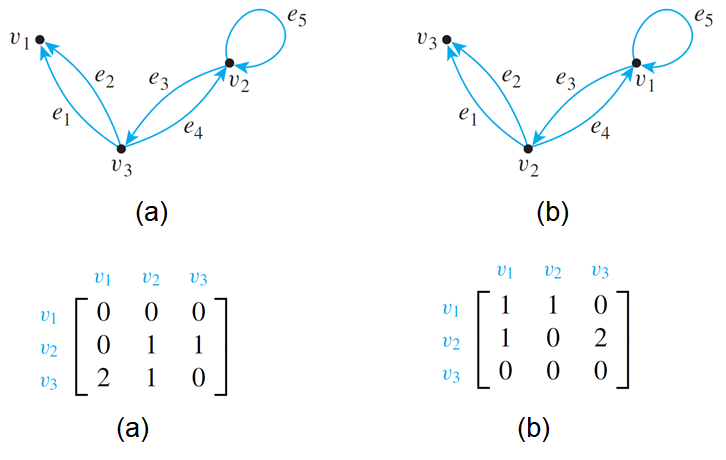
\includegraphics[width=1\linewidth]{screenshot001}
				
				\item [Adjacency Matrix of an Undirected Graph]:\\
				Let $G$ be an undirected graph with ordered vertices $v_1,v_2,...,v_n$. The \textbf{adjacency matrix of $G$} is the $n\times n$ matrix $A = a_{ij})$ over the set of non-negative integers s.t.\\
				$a_{ij} =$ the number of edges connecting $v_i$ and $v_j$\\ 
				$\forall i,j=1,2,...,n$.\\
				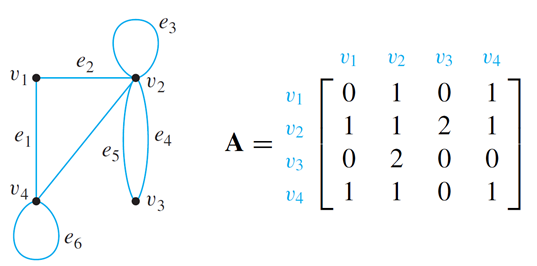
\includegraphics[width=1\linewidth]{screenshot002}
				PS: The matrix is \textbf{symmetric}
				
				\item [Symmetric Matrix]:\\
				An $n\times n$ square matrix $A = (a_{ij})$ is called \textbf{symmetric} iff $a_{ij}=a_{ji}, \forall i,j = 1, 2,..., n$
				\columnbreak
				\item [Thm 10.3.1]:\\
				Let $G$ be a graph with connected components $G_1, G_2, ..., G_k$. If there are $n_i$ vertices in each connected component $G_i$ and these vertices are numbered consecutively, then the adjacency matrix of $G$ has the form:\\
				$\begin{bmatrix}
				A_1 & 0 & 0 & & 0 & 0\\
				0 & A_2 & 0 & ... & 0 & 0 \\
				0 & 0 & A_3 & & 0 & 0\\
				& \vdots & & & \vdots & \vdots\\
				0 & 0 & 0 & ... & 0 & A_k
				\end{bmatrix}$\\
				where each $A_i$ is $n_i\times n_i$ adjacency matrix of $G_i$, $\forall i = 1, 2,..., k$, and the $0$’s represent matrices whose entries are all $0$'s.
				
				\item [and so on...]
			\end{descitemize}
\end{multicols*}
\end{document}